\documentclass[final,3p,times,authoryear]{elsarticle}

\usepackage{graphicx}
\usepackage{amsmath}
\usepackage{amssymb}
\usepackage{algorithm}
\usepackage{algorithmic}
\usepackage{booktabs}
\usepackage{multirow}
\usepackage{url}
\usepackage{hyperref}
\usepackage{tikz}
\usetikzlibrary{shapes,arrows,positioning,calc,shapes.geometric,decorations.pathreplacing}
\usepackage{pgfplots}
\pgfplotsset{compat=1.18}
\usepackage{pifont}
\usepackage{float}
\usepackage{tabularx}
\usepackage{array}
\usepackage{adjustbox}
\usepackage{xurl}
\usepackage{seqsplit}
\sloppy
\newcolumntype{Y}{>{\raggedright\arraybackslash}X}

\journal{ACM Transactions on Computer-Human Interaction}

\begin{document}

\begin{frontmatter}

\title{Beyond One-Size-Fits-All: A Memory-Aware Agentic Interview Framework with Joint Adaptive Control and Selection, Session-Level Report Analysis, and Learner-Centered Evaluation}

\author{Anonymous Authors}

\begin{abstract}
\noindent Adaptive technical interviewing is a sequential decision problem: given incomplete observations of a candidate's ability, a limited question budget, and noisy evaluation signals, the system must decide what to ask next, when to follow up, and when to stop. We formulate this problem as a closed-loop observation--memory--policy--action process and present a domain-specific, memory-aware, tool-augmented adaptive interview framework with structured control logic and constrained LLM usage. At each turn the framework maintains persistent interview memory encoding performance history, coverage state, knowledge gaps, resume-derived priors, and evaluator feedback; compresses this memory into a structured state representation; and invokes a planner/controller that selects an action from a constrained action space $a_t \in \{\textit{ask-next}, \textit{follow-up}, \textit{terminate}\}$. The controller dispatches actions through a tool router that invokes specialized modules---rule-based scoring, validated LLM judging, follow-up generation, resume parsing, and report synthesis---each operating under reliability constraints with automatic fallback. We contribute four elements: (C1)~a memory-aware agentic interview framework with an observation--memory--policy--action loop; (C2)~a \emph{joint adaptive policy under budget constraints} that couples difficulty calibration and termination with state-conditioned, evaluator-informed question selection; (C3)~a \emph{session-level analytical report pipeline} that decomposes the full interview trace into granular signals and runs sequential analysis steps with rule-based fallback; and (C4)~a learner-centered, psychometrically motivated evaluation protocol for AI interview systems. On the current offline project dataset, the system achieves 80.6\% calibration accuracy, 93.1\% uptime, and 4.2/5.0 satisfaction, but system--human scoring agreement remains weak on correctness, depth, tradeoff reasoning, and overall score. These results position the prototype as a training and feedback system rather than a standalone hiring decision system, and they identify scoring calibration as the main target for future improvement.
\end{abstract}

\begin{keyword}
Agentic AI \sep Interview agents \sep Adaptive assessment \sep Joint adaptive policy \sep Session-level report analysis \sep Tool-augmented LLM systems \sep Memory-aware interaction \sep Learner-centered evaluation
\end{keyword}

\end{frontmatter}

%% ============================================================
%%  SECTION 1: INTRODUCTION
%% ============================================================
\section{Introduction}

\subsection{Adaptive Interviewing as a Sequential Decision Problem}

\noindent Technical interviews are a cornerstone of hiring in software engineering, yet they remain a source of stress and inequity for candidates \cite{kim2024interview}. AI-powered systems promise to scale assessment consistently, but most simply replicate existing problems at scale: fixed difficulty, generic question sequences, and evaluation that is either shallow or unreliable.

We argue that adaptive technical interviewing is fundamentally a \emph{sequential decision problem under limited question budgets, incomplete observations, and reliability constraints}. At each turn $t$, the system observes a candidate response, updates its beliefs about candidate ability and knowledge state, and must choose the next action---ask a new question, probe deeper with a follow-up, or terminate the interview---subject to budget and coverage constraints. This formulation exposes three design gaps that limit current systems.

\noindent \textbf{Problem 1: Inconsistent difficulty calibration.} Traditional interviews employ fixed difficulty levels that may be too challenging for some candidates while insufficiently challenging for others, leading to inaccurate ability estimation and poor candidate experience \cite{van2006computerized}. In AI-powered systems, the problem persists: most platforms use fixed templates or simple rule-based adjustments that lack rapid calibration within the limited question counts typical of technical interviews \cite{kim2024interview}. The system's difficulty controller must converge quickly under a constrained question budget, yet existing CAT methods require extensive calibration data and more items than a practical interview allows \cite{van2006computerized}.

\noindent \textbf{Problem 2: Context-blind question selection.} Current approaches either employ random selection, which fails to target knowledge gaps, or use rigid templates that ignore candidate backgrounds and performance history \cite{chen2022personalization}. Question selection must simultaneously address identified weaknesses, ensure coverage across knowledge domains, and personalize based on resume-derived priors, yet existing systems rarely integrate these signals into a unified selection policy \cite{li2022resume,vanlehn2011relative}.

\noindent \textbf{Problem 3: Reliability--nuance trade-off in evaluation.} Rule-based evaluation provides consistent scoring but lacks nuanced understanding \cite{patel2023reliability,burrows2015eraser}. Purely LLM-based evaluation offers sophisticated analysis but introduces variability and external service dependency \cite{chang2023survey,zhang2023evaluation}. In a high-stakes assessment context, the judging subsystem must route between deterministic and LLM-based evaluation, validate outputs, and fall back gracefully when external services fail.

\subsection{Existing Methods and Their Limitations}

\noindent Several research strands have attempted to address these problems, yet each falls short for technical interview contexts.

\noindent \textbf{Difficulty calibration.} Computerized adaptive testing (CAT) has addressed difficulty calibration through Item Response Theory (IRT) and ability estimation algorithms \cite{van2006computerized,chen2021adaptive}. However, CAT approaches require extensive calibration data and typically need more questions than a practical interview allows to stabilize difficulty \cite{van2006computerized}. They do not account for interview-specific constraints such as multi-dimensional scoring, follow-up decisions, or coverage requirements.

\noindent \textbf{Question selection.} Intelligent tutoring systems employ adaptive algorithms for personalized learning and question selection \cite{vanlehn2011relative}, but focus on instruction rather than assessment. Recent work on personalized question selection \cite{chen2022personalization} has shown promise, but integration with candidate background information remains limited \cite{li2022resume}. No existing framework unifies gap targeting, resume priors, coverage maximization, and evaluator feedback into a single state-conditioned policy.

\noindent \textbf{Evaluation.} Modern language models have shown remarkable evaluation capabilities \cite{brown2020gpt3,achiam2023gpt4}, and instruction-tuned models demonstrate improved reliability \cite{ouyang2022chatgpt}. However, rule-based systems struggle with semantic understanding, while LLM systems face consistency challenges \cite{chang2023survey}. Hybrid approaches remain underexplored in technical interview contexts where both reliability and graceful degradation are essential \cite{smith2021hybrid}.

\subsection{Our Solution and Contributions}

\noindent We present a \emph{domain-specific, memory-aware, tool-augmented adaptive interview framework} that addresses the three design gaps through a formal agentic formulation. We model the interview as a closed-loop process:
\begin{equation}
o_t \;\rightarrow\; m_t \;\rightarrow\; s_t \;\rightarrow\; \pi(a_t \mid s_t) \;\rightarrow\; \text{tool use} \;\rightarrow\; \text{feedback} \;\rightarrow\; m_{t+1},\; s_{t+1}
\label{eq:agentic_loop}
\end{equation}
where $o_t$ is the observation (candidate response + evaluation signals), $m_t$ is persistent interview memory, $s_t$ is the compressed state, $\pi$ is the planner/controller policy, and $a_t \in \{\textit{ask-next},\, \textit{follow-up},\, \textit{terminate}\}$ is the action. The controller dispatches actions through a tool router that invokes specialized modules under reliability constraints with automatic fallback.

We emphasize that this is an \emph{agentic orchestration framework} with structured control logic---not an unconstrained autonomous agent. The action space is fixed, the control policy is deterministic and auditable, and LLM components operate under validation and fallback constraints. This design prioritizes reproducibility and reliability over open-ended autonomy, consistent with the requirements of high-stakes assessment.

\noindent \textbf{Research Questions.} This research addresses three fundamental questions:

\textbf{RQ1:} How can a \emph{joint adaptive policy} couple difficulty calibration and budget-constrained termination with state-conditioned question selection---including gap targeting, resume priors, coverage, evaluator next-direction hints $\eta_t$, and optional LLM-as-topic planning---so that both control and selection read from the same persistent memory and can be evaluated under a small interview question budget without pre-calibrated IRT item parameters?

\textbf{RQ2:} How can a \emph{session-level analytical report pipeline} decompose the full interview trace (per-turn questions, responses, scores, trajectories, and gaps) and analyze it through multiple complementary lenses---summative narrative, dimensional attribution, diagnostic gap analysis, actionable learning guidance, and transparent strategy explanation---with step-wise reliability (rule fallbacks)?

\textbf{RQ3:} What \emph{learner-centered outcomes} (e.g., perceived usefulness, readiness/confidence, fairness, intent to reuse) do students or candidates experience when using the system, and how do these compare to prior HCI studies of AI mock interviews \cite{conversate2024,virtual_interviewers2025}?

\noindent \textbf{Contributions.} We make four primary contributions (C1--C4):
\begin{itemize}
    \item \textbf{C1 (Framework)}: A memory-aware agentic interview framework with an observation--memory--policy--action loop that formulates adaptive interviewing as a sequential decision process with persistent state, structured tool invocation, and feedback-driven memory updates (Section~\ref{sec:method}).
    \item \textbf{C2 (Joint adaptive policy)}: A budget-constrained \emph{joint} adaptive policy that couples Sections~\ref{sec:adaptive_control} and~\ref{sec:selection}: the same interview memory drives sliding-window difficulty/termination control and multi-objective, evaluator-informed question selection (including LLM-as-topic-planner with priority/Fisher/UCB fallbacks), closing an evaluation-to-selection loop via $\eta_t$.
    \item \textbf{C3 (Session-level report analysis)}: A multi-step report pipeline that ingests the full session, compresses it into structured context, and runs five sequential analysis steps with independent fallbacks (Section~\ref{sec:report_pipeline}, Tables~\ref{tab:report_decomposition}--\ref{tab:report_steps}).
    \item \textbf{C4 (Evaluation protocol)}: A learner-centered and psychometrically motivated evaluation protocol that combines CAT-style calibration, question-selection diagnostics, system--human scoring validity, human inter-rater reliability, satisfaction, subgroup diagnostics, and offline rollout gates (Sections~\ref{sec:experiments}--\ref{sec:results}).
\end{itemize}

The remainder of this paper is organized as follows. Section~\ref{sec:related} reviews related work and positions our contribution. Section~\ref{sec:method} presents the agentic method framework, including problem formulation, memory/state design, controller, joint adaptive policy (Sections~\ref{sec:adaptive_control}--\ref{sec:selection}), hybrid judging as the online evaluation module (Section~\ref{sec:hybrid_judging}), and session-level report synthesis (Section~\ref{sec:tools}). Section~\ref{sec:implementation} describes implementation details. Section~\ref{sec:experiments} presents experimental design, and Section~\ref{sec:results} reports results. Section~\ref{sec:discussion} discusses findings, limitations, and future work. Section~\ref{sec:conclusion} concludes.

%% ============================================================
%%  SECTION 2: RELATED WORK
%% ============================================================
\section{Related Work}
\label{sec:related}

\subsection{Computerized Adaptive Testing}

\noindent Researchers have extensively studied Computerized Adaptive Testing (CAT) in educational assessment contexts \cite{van2006computerized}. Recent surveys from a machine learning perspective synthesize measurement models, item selection algorithms, bank construction, and test control \cite{zhuang2024catsurvey}. The classical principle involves dynamically adjusting difficulty based on candidate responses, often grounded in Item Response Theory (IRT) \cite{hambleton1991fundamentals}. ROAR-CAT \cite{roarcat2025} demonstrates a gold-standard CAT development pipeline: IRT parameter estimation on 1,960 students, followed by validation with 485 students, achieving 40\% efficiency gains. However, many CAT variants rely on pre-calibrated item parameters and response models that do not directly apply to technical interviews, where items are heterogeneous, scoring is multi-dimensional, and \emph{item selection must be coupled with interview-specific termination and coverage constraints}. Our work targets the interview setting by proposing a lightweight joint policy: the same persistent memory conditions both difficulty/termination and multi-objective selection (including evaluator-informed hints), without assuming pre-calibrated IRT parameters, converging within a small number of questions under a fixed budget.

\subsection{Intelligent Tutoring Systems}

\noindent Intelligent Tutoring Systems (ITS) employ adaptive algorithms to personalize learning experiences based on student performance and knowledge gaps \cite{vanlehn2011relative}. While ITS share adaptive principles with assessment systems, their question selection prioritizes learning objectives over comprehensive evaluation. Our joint policy addresses RQ1 by balancing learning-oriented gap targeting with assessment-oriented coverage requirements, treating control and selection as co-dependent decisions over persistent interview state.

\subsection{AI-Powered Interview Systems and HCI}

\noindent Prior work has explored AI support for interviews and assessment \cite{kim2024interview,wang2023survey}. Conversate \cite{conversate2024} uses LLM-driven interactive simulation with adaptive follow-up questions; a 19-participant study found that adaptive follow-ups enhanced realism. Virtual Interviewers \cite{virtual_interviewers2025} report formative evidence on mock technical interviews, linking AI-driven practice to student readiness and confidence---themes we revisit under RQ3 (learner-centered outcomes). A modular AI interviewer \cite{modular_interviewer2025} with local LLMs achieved high satisfaction (4.45/5). From an HCI perspective, candidate experience and perceived fairness are critical \cite{kumar2022fairness}. Multimodal approaches integrating text, audio, and video analysis have shown promise \cite{wang2022multimodal}. However, few systems formalize adaptive interviewing as a memory-aware sequential decision process with a \emph{joint} control-and-selection policy, structured tool invocation, reliability-constrained online judging, session-level multi-step report analysis, and feedback-driven state updates.

\subsection{LLM Agents, Tool-Augmented Workflows, and Memory-Augmented Systems}
\label{sec:related_agents}

\noindent Recent advances in LLM agents have shifted from single-model prompting toward autonomous systems that reason, plan, and execute multi-step tasks \cite{llm_agent_survey2025,wang2023survey}. ReAct \cite{yao2023react} introduced the Thought--Action--Observation loop, combining explicit reasoning with tool execution. Agentic workflows integrate multiple specialized components with orchestration logic and tool-augmented capabilities \cite{agentic_workflow_guide2025}. Automated workflow generation \cite{aflow2024} has explored search-based optimization over code-represented workflows.

\emph{Tool-augmented} LLM agents extend model capabilities by invoking external tools (calculators, retrievers, code interpreters) through structured APIs. This paradigm separates the planner from the executor, enabling modular, testable tool pipelines. Our framework adopts this principle: the interview controller is a structured planner that invokes specialized tools (rule-based scorer, LLM judge, follow-up generator, resume parser) through a tool router, rather than delegating all reasoning to a single LLM.

\emph{Memory-augmented} agent architectures maintain persistent state across interaction turns, enabling context-aware decisions that depend on the full interaction history rather than a single prompt window. Our interview memory (Section~\ref{sec:memory}) is a domain-specific instance of this pattern, encoding score trajectories, coverage state, knowledge gaps, and evaluator hints across turns.

Our framework differs from general-purpose LLM agents in three key ways: (i)~the action space is \emph{constrained} to $\{\textit{ask-next}, \textit{follow-up}, \textit{terminate}\}$, preventing unconstrained generation; (ii)~the control logic is \emph{deterministic and auditable}, using reproducible algorithms rather than free-form LLM reasoning; and (iii)~the system enforces \emph{graceful fallback} under LLM failure, ensuring reliability in high-stakes assessment contexts. These properties distinguish our work from ReAct-style agents where the LLM controls both planning and execution.

\subsection{LLM-as-a-Judge and Reliability-Aware Evaluation}

\noindent The LLM-as-a-judge paradigm uses language models to evaluate outputs, with growing adoption in assessment and benchmarking \cite{chang2023survey,zhang2023evaluation}. A meta-analysis of 65 LLM-based automated scoring studies \cite{llm_aes_meta2025} reports agreement indices (QWK, Pearson $r$) mostly in the 0.30--0.80 range, with substantial variability. Targeted formative assessment studies \cite{llm_formative2025} show that context-enhanced few-shot chain-of-thought prompting improves LLM--human agreement. An AI-driven mock interview study \cite{ai_mock_ijmlc2025} found that LLMs approach human-level agreement on technical questions.

However, reliability-aware evaluation requires more than a single LLM call. \emph{Multi-judge aggregation} reduces variance by running multiple independent LLM evaluations and combining scores \cite{zhang2023evaluation}. \emph{Judge routing} selects between rule-based and LLM judges based on input characteristics and availability. \emph{Validation and fallback} ensures that malformed or out-of-range LLM outputs are caught and replaced by deterministic alternatives. Our hybrid judging framework (Section~\ref{sec:hybrid_judging}) combines all three mechanisms, providing reliability-constrained evaluation with provenance tracking.

\subsection{Natural Language Processing for Assessment}

\noindent Text similarity and semantic analysis techniques have been applied to automated answer evaluation \cite{burrows2015eraser,mohler2011evaluation}. Pre-trained language models enable stronger semantic representations \cite{devlin2018bert}, and prompt engineering techniques including chain-of-thought reasoning \cite{wei2022chain} further improve evaluation quality. Our hybrid evaluator combines a deterministic rule-based baseline with optional LLM augmentation and validation, operating as a tool within the agentic framework rather than as a standalone scoring module.

%% ============================================================
%%  SECTION 3: METHOD
%% ============================================================
\section{Method: Memory-Aware Agentic Interview Framework}
\label{sec:method}

This section presents the core method. We first formalize the problem (Section~\ref{sec:formulation}), then define the observation, memory, and state representations (Sections~\ref{sec:observation}--\ref{sec:state}). We introduce the planner/controller (Section~\ref{sec:controller}) and detail the \emph{joint adaptive policy} in two parts---adaptive control (Section~\ref{sec:adaptive_control}) and state-aware selection (Section~\ref{sec:selection})---followed by follow-up planning (Section~\ref{sec:followup}). The reliability-constrained hybrid judge (Section~\ref{sec:hybrid_judging}) is the online evaluation module that produces structured scores and $\eta_t$ for memory. We conclude with the tool-augmented architecture and session-level report pipeline (Section~\ref{sec:tools}).

\subsection{Problem Formulation}
\label{sec:formulation}

\noindent We formulate adaptive technical interviewing as a memory-aware sequential decision process. Let $t = 1, 2, \ldots$ index interview turns. At each turn:

\begin{itemize}
    \item The system presents question $q_t$ at difficulty $d_t$ from chapter $c_t$.
    \item The candidate produces response $y_t$.
    \item The hybrid judge produces evaluation output $e_t = (S_t, M_t^{\text{new}}, \eta_t)$, where $S_t$ is the multi-dimensional score vector, $M_t^{\text{new}}$ is the set of newly identified missing concepts, and $\eta_t$ is the optional next-direction hint.
    \item The system updates interview memory $m_t$ and state $s_t$.
    \item The planner/controller selects action $a_t \in \{\textit{ask-next},\, \textit{follow-up},\, \textit{terminate}\}$.
\end{itemize}

The process follows the closed-loop formulation in Eq.~\eqref{eq:agentic_loop}. The controller's objective is to maximize assessment validity (accurate ability estimation, comprehensive coverage, targeted gap identification) subject to a budget constraint $t \leq B$, where $B$ is derived from the user-specified round count $r_{\text{user}}$ and adaptive bounds (Section~\ref{sec:adaptive_control}).

\subsection{Observation}
\label{sec:observation}

\noindent At each turn $t$, the observation $o_t$ consists of:
\begin{equation}
o_t = (q_t, y_t, e_t) = \bigl(q_t,\; y_t,\; (S_t, M_t^{\text{new}}, \eta_t)\bigr)
\end{equation}
where $q_t$ is the presented question (with its difficulty $d_t$ and chapter $c_t$), $y_t$ is the candidate's response (text and/or transcribed audio), and $e_t$ is the structured evaluation output from the hybrid judge. The evaluation $e_t$ includes five-dimensional scores $S_t = (s_t^{\text{corr}}, s_t^{\text{depth}}, s_t^{\text{clar}}, s_t^{\text{prac}}, s_t^{\text{trade}})$, an overall score $s_t$, newly identified missing concepts $M_t^{\text{new}}$, textual feedback, and an optional LLM-generated next-direction hint $\eta_t$.

\subsection{Interview Memory}
\label{sec:memory}

\noindent Interview memory $m_t$ is a persistent data structure that accumulates information across turns. After turn $t$, the memory contains:

\begin{equation}
m_t = \bigl(\mathcal{H}_t,\; \mathcal{S}_t,\; \mathcal{D}_t,\; \mathcal{C}_t,\; \mathcal{M}_t,\; R,\; \mathcal{F}_t,\; \mathcal{E}_t\bigr)
\end{equation}

where:
\begin{itemize}
    \item $\mathcal{H}_t = \{(q_i, y_i, e_i)\}_{i=1}^{t}$ is the interaction history (all question--response--evaluation triples).
    \item $\mathcal{S}_t = \{s_i\}_{i=1}^{t}$ is the score history (overall scores per turn).
    \item $\mathcal{D}_t = \{d_i\}_{i=1}^{t}$ is the difficulty trajectory.
    \item $\mathcal{C}_t = \{c_i\}_{i=1}^{t}$ is the chapter coverage trace (which chapters have been visited).
    \item $\mathcal{M}_t = \bigcup_{i=1}^{t} M_i^{\text{new}}$ is the accumulated set of missing concepts / misconceptions.
    \item $R$ is the resume-derived prior (parsed skills, experience, projects), fixed at session start.
    \item $\mathcal{F}_t$ is the follow-up trace (which questions received follow-ups, how many, and outcomes).
    \item $\mathcal{E}_t = \{\eta_i\}_{i=1}^{t}$ is the sequence of evaluator next-direction hints.
\end{itemize}

Memory is updated after each turn: $m_{t+1} = \textsc{Update}(m_t, o_t)$. This update appends the new observation to the history, extends the score/difficulty/coverage traces, merges new missing concepts into the accumulated set, and records any follow-up decisions.

% ================= Figure 4: Memory State =================
\begin{figure*}[t]
\centering
\resizebox{\textwidth}{!}{% Composition and Update of Persistent Interview Memory
% Use with: % Composition and Update of Persistent Interview Memory
% Use with: % Composition and Update of Persistent Interview Memory
% Use with: \input{figures/memory_state.tex}

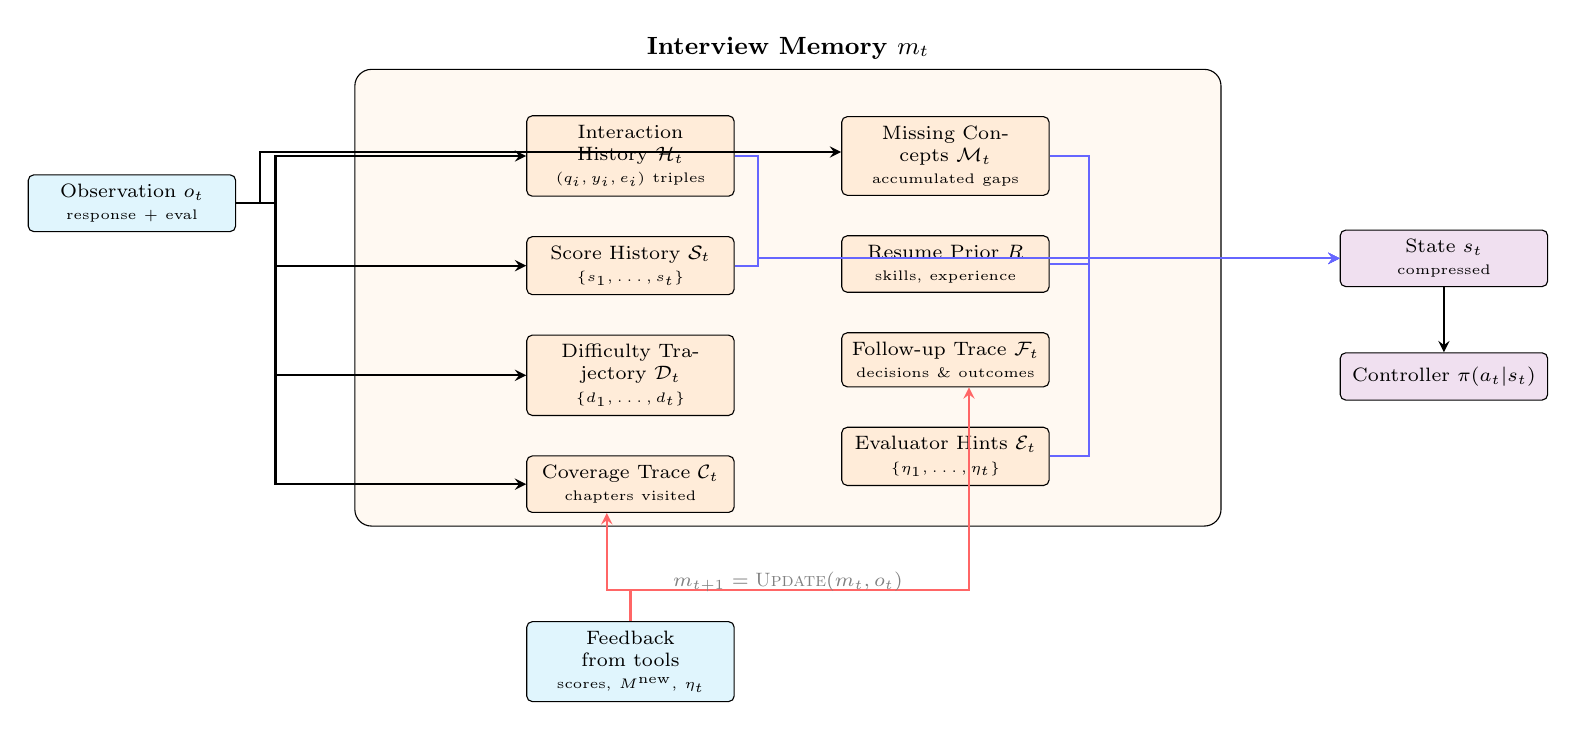
\begin{tikzpicture}[
    node distance=0.5cm and 0.6cm,
    slot/.style={rectangle, draw, rounded corners=2pt, minimum height=0.6cm, text centered, font=\scriptsize, text width=2.4cm},
    mem/.style={slot, fill=orange!15},
    inp/.style={slot, fill=cyan!12},
    outp/.style={slot, fill=violet!12},
    arr/.style={->, >=stealth, thick},
    darr/.style={->, >=stealth, thick, dashed, gray!60},
]

% === Memory box ===
\node[draw, rounded corners=6pt, fill=orange!5, minimum width=11cm, minimum height=5.8cm, label={[font=\small\bfseries]above:Interview Memory $m_t$}] (membox) {};

% === Memory slots (2 columns inside membox) ===
\node[mem] (h) at ([xshift=-2cm, yshift=1.8cm]membox.center) {Interaction History $\mathcal{H}_t$\\{\tiny $(q_i, y_i, e_i)$ triples}};
\node[mem, below=of h] (s) {Score History $\mathcal{S}_t$\\{\tiny $\{s_1, \ldots, s_t\}$}};
\node[mem, below=of s] (d) {Difficulty Trajectory $\mathcal{D}_t$\\{\tiny $\{d_1, \ldots, d_t\}$}};
\node[mem, below=of d] (c) {Coverage Trace $\mathcal{C}_t$\\{\tiny chapters visited}};

\node[mem] (m) at ([xshift=2cm, yshift=1.8cm]membox.center) {Missing Concepts $\mathcal{M}_t$\\{\tiny accumulated gaps}};
\node[mem, below=of m] (r) {Resume Prior $R$\\{\tiny skills, experience}};
\node[mem, below=of r] (f) {Follow-up Trace $\mathcal{F}_t$\\{\tiny decisions \& outcomes}};
\node[mem, below=of f] (e) {Evaluator Hints $\mathcal{E}_t$\\{\tiny $\{\eta_1, \ldots, \eta_t\}$}};

% === Input: Observation ===
\node[inp, left=1.5cm of membox.west, yshift=1.2cm] (obs) {Observation $o_t$\\{\tiny response + eval}};

% === Output: State ===
\node[outp, right=1.5cm of membox.east, yshift=0.5cm] (state) {State $s_t$\\{\tiny compressed}};

% === Output: Controller ===
\node[outp, right=1.5cm of membox.east, yshift=-1.0cm] (ctrl) {Controller $\pi(a_t|s_t)$};

% === Arrows: Observation updates memory ===
\draw[arr] (obs.east) -- ++(0.5,0) |- (h.west);
\draw[arr] (obs.east) -- ++(0.5,0) |- (s.west);
\draw[arr] (obs.east) -- ++(0.5,0) |- (d.west);
\draw[arr] (obs.east) -- ++(0.5,0) |- (c.west);
\draw[arr] (obs.east) -- ++(0.3,0) |- ([yshift=0.05cm]m.west);

% === Arrows: Memory -> State (compress) ===
\draw[arr, blue!60] (h.east) -- ++(0.3,0) |- (state.west);
\draw[arr, blue!60] (s.east) -- ++(0.3,0) |- (state.west);
\draw[arr, blue!60] (m.east) -- ++(0.5,0) |- (state.west);
\draw[arr, blue!60] (r.east) -- ++(0.5,0) |- (state.west);
\draw[arr, blue!60] (e.east) -- ++(0.5,0) |- (state.west);

% State -> Controller
\draw[arr] (state) -- (ctrl);

% === Feedback loop annotation ===
\node[inp, below=1.2cm of membox.south, xshift=-2cm] (feedback) {Feedback from tools\\{\tiny scores, $M^{\text{new}}$, $\eta_t$}};
\draw[arr, red!60, thick] (feedback.north) -- ++(0,0.4) -| ([xshift=-0.3cm]c.south);
\draw[arr, red!60, thick] (feedback.north) -- ++(0,0.4) -| ([xshift=0.3cm]f.south);

% Update label
\node[font=\scriptsize\itshape, gray] at ([yshift=-0.7cm]membox.south) {$m_{t+1} = \textsc{Update}(m_t, o_t)$};

\end{tikzpicture}


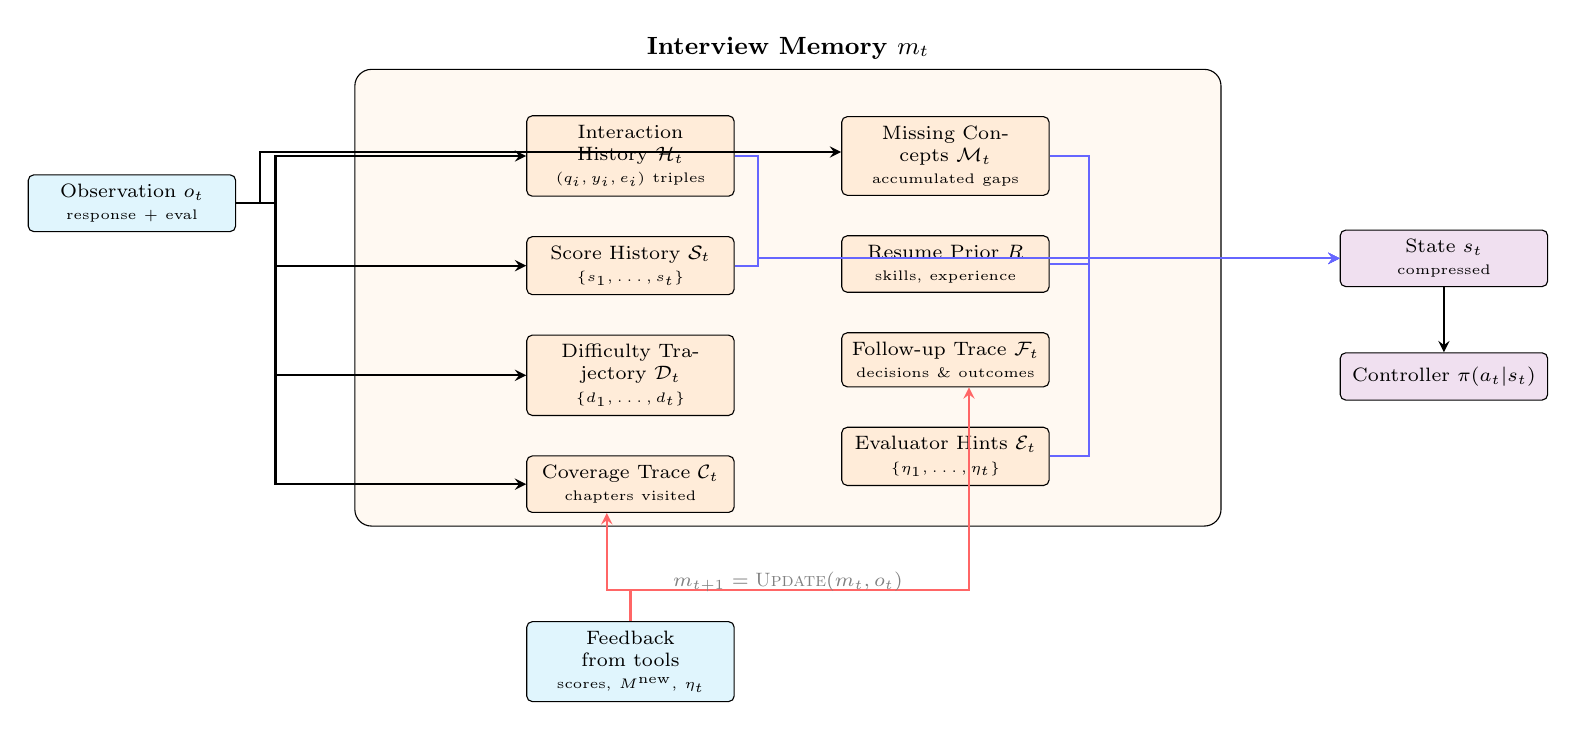
\begin{tikzpicture}[
    node distance=0.5cm and 0.6cm,
    slot/.style={rectangle, draw, rounded corners=2pt, minimum height=0.6cm, text centered, font=\scriptsize, text width=2.4cm},
    mem/.style={slot, fill=orange!15},
    inp/.style={slot, fill=cyan!12},
    outp/.style={slot, fill=violet!12},
    arr/.style={->, >=stealth, thick},
    darr/.style={->, >=stealth, thick, dashed, gray!60},
]

% === Memory box ===
\node[draw, rounded corners=6pt, fill=orange!5, minimum width=11cm, minimum height=5.8cm, label={[font=\small\bfseries]above:Interview Memory $m_t$}] (membox) {};

% === Memory slots (2 columns inside membox) ===
\node[mem] (h) at ([xshift=-2cm, yshift=1.8cm]membox.center) {Interaction History $\mathcal{H}_t$\\{\tiny $(q_i, y_i, e_i)$ triples}};
\node[mem, below=of h] (s) {Score History $\mathcal{S}_t$\\{\tiny $\{s_1, \ldots, s_t\}$}};
\node[mem, below=of s] (d) {Difficulty Trajectory $\mathcal{D}_t$\\{\tiny $\{d_1, \ldots, d_t\}$}};
\node[mem, below=of d] (c) {Coverage Trace $\mathcal{C}_t$\\{\tiny chapters visited}};

\node[mem] (m) at ([xshift=2cm, yshift=1.8cm]membox.center) {Missing Concepts $\mathcal{M}_t$\\{\tiny accumulated gaps}};
\node[mem, below=of m] (r) {Resume Prior $R$\\{\tiny skills, experience}};
\node[mem, below=of r] (f) {Follow-up Trace $\mathcal{F}_t$\\{\tiny decisions \& outcomes}};
\node[mem, below=of f] (e) {Evaluator Hints $\mathcal{E}_t$\\{\tiny $\{\eta_1, \ldots, \eta_t\}$}};

% === Input: Observation ===
\node[inp, left=1.5cm of membox.west, yshift=1.2cm] (obs) {Observation $o_t$\\{\tiny response + eval}};

% === Output: State ===
\node[outp, right=1.5cm of membox.east, yshift=0.5cm] (state) {State $s_t$\\{\tiny compressed}};

% === Output: Controller ===
\node[outp, right=1.5cm of membox.east, yshift=-1.0cm] (ctrl) {Controller $\pi(a_t|s_t)$};

% === Arrows: Observation updates memory ===
\draw[arr] (obs.east) -- ++(0.5,0) |- (h.west);
\draw[arr] (obs.east) -- ++(0.5,0) |- (s.west);
\draw[arr] (obs.east) -- ++(0.5,0) |- (d.west);
\draw[arr] (obs.east) -- ++(0.5,0) |- (c.west);
\draw[arr] (obs.east) -- ++(0.3,0) |- ([yshift=0.05cm]m.west);

% === Arrows: Memory -> State (compress) ===
\draw[arr, blue!60] (h.east) -- ++(0.3,0) |- (state.west);
\draw[arr, blue!60] (s.east) -- ++(0.3,0) |- (state.west);
\draw[arr, blue!60] (m.east) -- ++(0.5,0) |- (state.west);
\draw[arr, blue!60] (r.east) -- ++(0.5,0) |- (state.west);
\draw[arr, blue!60] (e.east) -- ++(0.5,0) |- (state.west);

% State -> Controller
\draw[arr] (state) -- (ctrl);

% === Feedback loop annotation ===
\node[inp, below=1.2cm of membox.south, xshift=-2cm] (feedback) {Feedback from tools\\{\tiny scores, $M^{\text{new}}$, $\eta_t$}};
\draw[arr, red!60, thick] (feedback.north) -- ++(0,0.4) -| ([xshift=-0.3cm]c.south);
\draw[arr, red!60, thick] (feedback.north) -- ++(0,0.4) -| ([xshift=0.3cm]f.south);

% Update label
\node[font=\scriptsize\itshape, gray] at ([yshift=-0.7cm]membox.south) {$m_{t+1} = \textsc{Update}(m_t, o_t)$};

\end{tikzpicture}


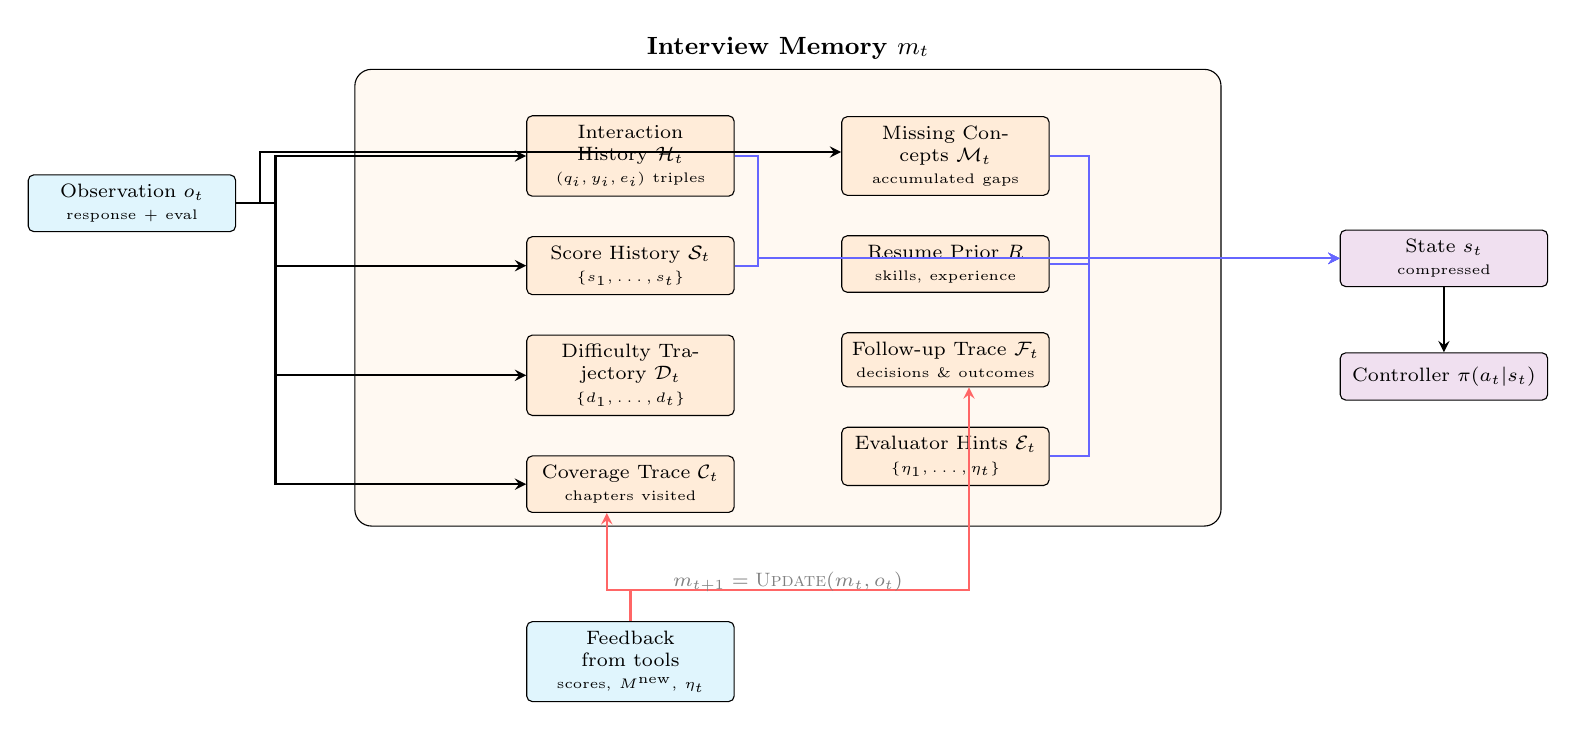
\begin{tikzpicture}[
    node distance=0.5cm and 0.6cm,
    slot/.style={rectangle, draw, rounded corners=2pt, minimum height=0.6cm, text centered, font=\scriptsize, text width=2.4cm},
    mem/.style={slot, fill=orange!15},
    inp/.style={slot, fill=cyan!12},
    outp/.style={slot, fill=violet!12},
    arr/.style={->, >=stealth, thick},
    darr/.style={->, >=stealth, thick, dashed, gray!60},
]

% === Memory box ===
\node[draw, rounded corners=6pt, fill=orange!5, minimum width=11cm, minimum height=5.8cm, label={[font=\small\bfseries]above:Interview Memory $m_t$}] (membox) {};

% === Memory slots (2 columns inside membox) ===
\node[mem] (h) at ([xshift=-2cm, yshift=1.8cm]membox.center) {Interaction History $\mathcal{H}_t$\\{\tiny $(q_i, y_i, e_i)$ triples}};
\node[mem, below=of h] (s) {Score History $\mathcal{S}_t$\\{\tiny $\{s_1, \ldots, s_t\}$}};
\node[mem, below=of s] (d) {Difficulty Trajectory $\mathcal{D}_t$\\{\tiny $\{d_1, \ldots, d_t\}$}};
\node[mem, below=of d] (c) {Coverage Trace $\mathcal{C}_t$\\{\tiny chapters visited}};

\node[mem] (m) at ([xshift=2cm, yshift=1.8cm]membox.center) {Missing Concepts $\mathcal{M}_t$\\{\tiny accumulated gaps}};
\node[mem, below=of m] (r) {Resume Prior $R$\\{\tiny skills, experience}};
\node[mem, below=of r] (f) {Follow-up Trace $\mathcal{F}_t$\\{\tiny decisions \& outcomes}};
\node[mem, below=of f] (e) {Evaluator Hints $\mathcal{E}_t$\\{\tiny $\{\eta_1, \ldots, \eta_t\}$}};

% === Input: Observation ===
\node[inp, left=1.5cm of membox.west, yshift=1.2cm] (obs) {Observation $o_t$\\{\tiny response + eval}};

% === Output: State ===
\node[outp, right=1.5cm of membox.east, yshift=0.5cm] (state) {State $s_t$\\{\tiny compressed}};

% === Output: Controller ===
\node[outp, right=1.5cm of membox.east, yshift=-1.0cm] (ctrl) {Controller $\pi(a_t|s_t)$};

% === Arrows: Observation updates memory ===
\draw[arr] (obs.east) -- ++(0.5,0) |- (h.west);
\draw[arr] (obs.east) -- ++(0.5,0) |- (s.west);
\draw[arr] (obs.east) -- ++(0.5,0) |- (d.west);
\draw[arr] (obs.east) -- ++(0.5,0) |- (c.west);
\draw[arr] (obs.east) -- ++(0.3,0) |- ([yshift=0.05cm]m.west);

% === Arrows: Memory -> State (compress) ===
\draw[arr, blue!60] (h.east) -- ++(0.3,0) |- (state.west);
\draw[arr, blue!60] (s.east) -- ++(0.3,0) |- (state.west);
\draw[arr, blue!60] (m.east) -- ++(0.5,0) |- (state.west);
\draw[arr, blue!60] (r.east) -- ++(0.5,0) |- (state.west);
\draw[arr, blue!60] (e.east) -- ++(0.5,0) |- (state.west);

% State -> Controller
\draw[arr] (state) -- (ctrl);

% === Feedback loop annotation ===
\node[inp, below=1.2cm of membox.south, xshift=-2cm] (feedback) {Feedback from tools\\{\tiny scores, $M^{\text{new}}$, $\eta_t$}};
\draw[arr, red!60, thick] (feedback.north) -- ++(0,0.4) -| ([xshift=-0.3cm]c.south);
\draw[arr, red!60, thick] (feedback.north) -- ++(0,0.4) -| ([xshift=0.3cm]f.south);

% Update label
\node[font=\scriptsize\itshape, gray] at ([yshift=-0.7cm]membox.south) {$m_{t+1} = \textsc{Update}(m_t, o_t)$};

\end{tikzpicture}
}
\caption{Composition and update of persistent interview memory. The agent maintains structured memory across turns, including performance history, coverage state, missing concepts, follow-up traces, resume priors, and evaluator hints, which together condition future actions.}
\label{fig:memory_state}
\end{figure*}

\subsection{State Representation}
\label{sec:state}

\noindent The controller operates on a compressed state $s_t$ derived from memory $m_t$. The state aggregates the information needed for action selection:

\begin{equation}
s_t = \bigl(d_t,\; C_t,\; \mathcal{M}_t,\; R,\; E_t,\; B_t\bigr)
\label{eq:state}
\end{equation}

where:
\begin{itemize}
    \item $d_t$ is the current difficulty estimate (output of the adaptive control mechanism).
    \item $C_t$ is the coverage state: which chapters have been visited, how many times, and which remain unvisited.
    \item $\mathcal{M}_t$ is the missing-concept state: the accumulated set of identified knowledge gaps.
    \item $R$ is the resume-derived prior (skills matched to chapters via fuzzy matching).
    \item $E_t$ is the latest evaluation feedback: the most recent score, trend, and next-direction hint $\eta_t$.
    \item $B_t$ is the remaining budget: how many questions remain before the budget cap, and whether termination conditions are met.
\end{itemize}

This state representation enables the controller to make informed decisions about question difficulty, chapter selection, follow-up necessity, and interview termination, all conditioned on the full interview history as compressed into $s_t$.

\subsection{Planner / Controller}
\label{sec:controller}

\noindent The planner/controller is the central decision component. At each turn, given state $s_t$, it selects an action:

\begin{equation}
a_t = \pi(s_t) \in \{\textit{ask-next},\, \textit{follow-up},\, \textit{terminate}\}
\end{equation}

The controller policy $\pi$ is implemented as structured, deterministic logic (not learned or LLM-generated), ensuring auditability and reproducibility. The decision procedure is:

\begin{enumerate}
    \item \textbf{Termination check}: evaluate whether termination conditions are met based on budget constraints, performance stability, and coverage (Section~\ref{sec:adaptive_control}). If yes, $a_t = \textit{terminate}$.
    \item \textbf{Follow-up check}: if the current question has not exhausted its follow-up budget and the evaluation indicates misconceptions or partial understanding, $a_t = \textit{follow-up}$ (Section~\ref{sec:followup}).
    \item \textbf{Ask-next}: otherwise, $a_t = \textit{ask-next}$. The controller invokes the adaptive control mechanism to update difficulty $d_{t+1}$ (Section~\ref{sec:adaptive_control}) and the selection policy to choose the next question $q_{t+1}$ (Section~\ref{sec:selection}).
\end{enumerate}

Each action is dispatched through a \emph{tool router} that invokes the appropriate specialized module (Section~\ref{sec:tools}).

% ================= Figure 1: Agentic Framework =================
\begin{figure*}[t]
\centering
\resizebox{\textwidth}{!}{% Overall Memory-Aware Agentic Interview Framework
% Use with: % Overall Memory-Aware Agentic Interview Framework
% Use with: % Overall Memory-Aware Agentic Interview Framework
% Use with: \input{figures/agentic_framework.tex}

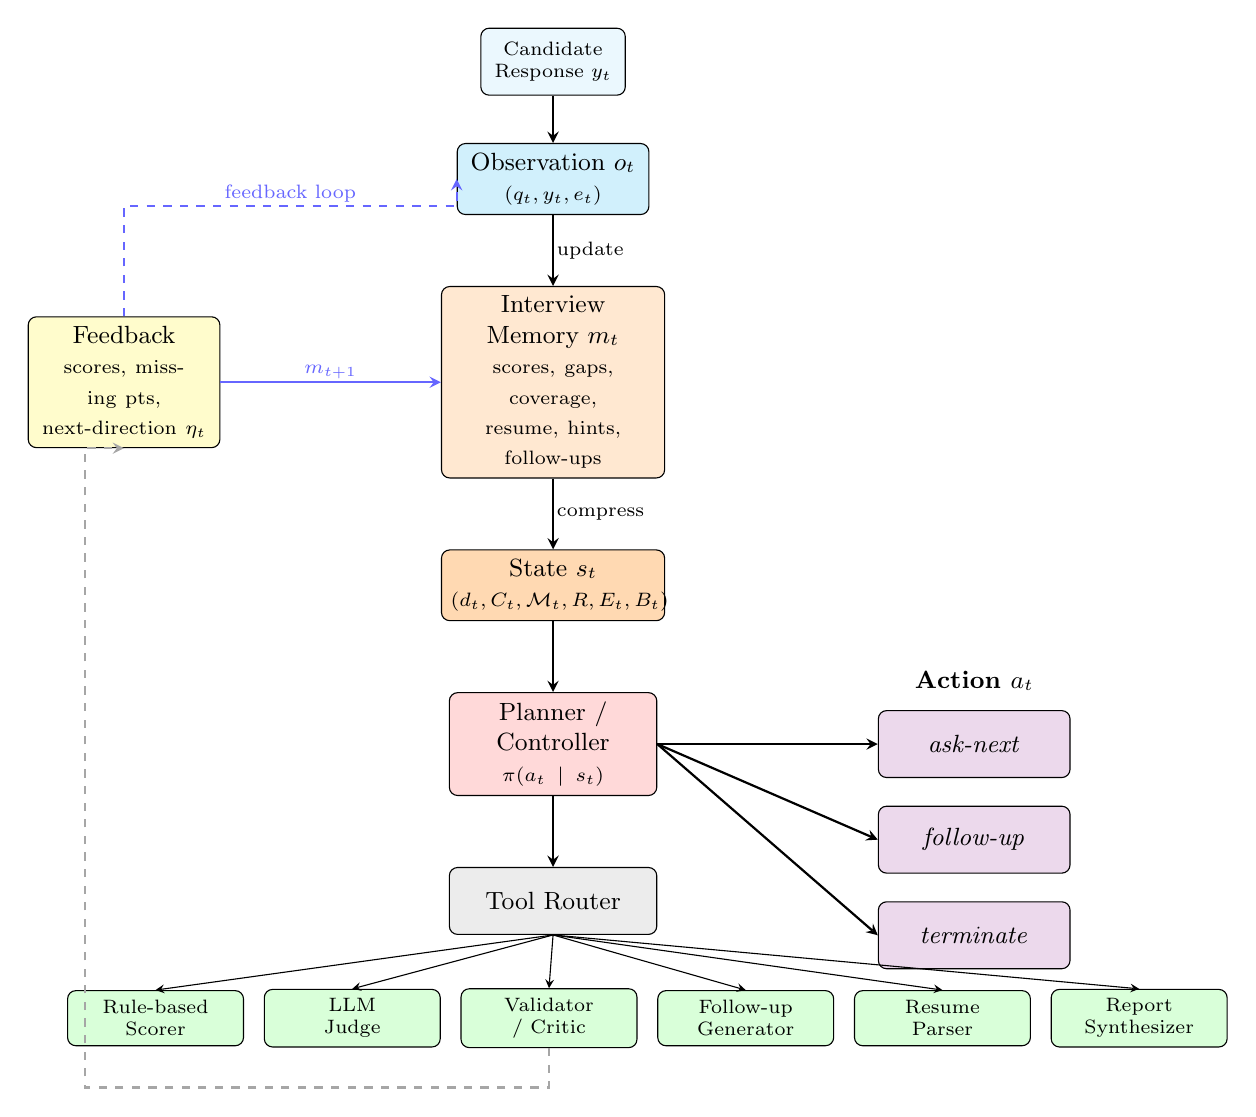
\begin{tikzpicture}[
    node distance=0.9cm and 1.2cm,
    block/.style={rectangle, draw, rounded corners=3pt, minimum height=0.85cm, text centered, font=\small},
    obs/.style={block, fill=cyan!18, text width=2.2cm},
    mem/.style={block, fill=orange!18, text width=2.6cm},
    ctrl/.style={block, fill=red!15, text width=2.4cm},
    tool/.style={block, fill=green!15, text width=2.0cm, minimum height=0.7cm, font=\scriptsize},
    act/.style={block, fill=violet!15, text width=2.2cm},
    fb/.style={block, fill=yellow!20, text width=2.2cm},
    arr/.style={->, >=stealth, thick},
    darr/.style={->, >=stealth, thick, dashed, gray!70},
    lbl/.style={font=\scriptsize, midway, fill=white, inner sep=1pt},
]

% === Row 1: Observation ===
\node[obs] (obs) {Observation $o_t$\\{\scriptsize $(q_t, y_t, e_t)$}};

% === Row 2: Memory ===
\node[mem, below=of obs] (mem) {Interview Memory $m_t$\\{\scriptsize scores, gaps, coverage,}\\{\scriptsize resume, hints, follow-ups}};

% === Row 3: State ===
\node[block, fill=orange!30, text width=2.6cm, below=of mem] (state) {State $s_t$\\{\scriptsize $(d_t, C_t, \mathcal{M}_t, R, E_t, B_t)$}};

% === Row 4: Controller ===
\node[ctrl, below=of state] (ctrl) {Planner / Controller\\{\scriptsize $\pi(a_t \mid s_t)$}};

% === Row 5: Tool Router ===
\node[block, fill=gray!15, text width=2.4cm, below=of ctrl, font=\small] (router) {Tool Router};

% === Tools (fanned below router) ===
\node[tool, below left=0.7cm and 2.6cm of router] (t1) {Rule-based\\Scorer};
\node[tool, right=0.25cm of t1] (t2) {LLM\\Judge};
\node[tool, right=0.25cm of t2] (t3) {Validator\\/ Critic};
\node[tool, right=0.25cm of t3] (t4) {Follow-up\\Generator};
\node[tool, right=0.25cm of t4] (t5) {Resume\\Parser};
\node[tool, right=0.25cm of t5] (t6) {Report\\Synthesizer};

% === Actions (right of controller) ===
\node[act, right=2.8cm of ctrl] (askn) {\textit{ask-next}};
\node[act, below=0.35cm of askn] (foll) {\textit{follow-up}};
\node[act, below=0.35cm of foll] (term) {\textit{terminate}};

% Action space label
\node[above=0.12cm of askn, font=\small\bfseries] {Action $a_t$};

% === Feedback (left of memory) ===
\node[fb, left=2.8cm of mem] (fb) {Feedback\\{\scriptsize scores, missing pts,}\\{\scriptsize next-direction $\eta_t$}};

% ===== Arrows =====
% Observation -> Memory
\draw[arr] (obs) -- node[lbl, right] {update} (mem);
% Memory -> State
\draw[arr] (mem) -- node[lbl, right] {compress} (state);
% State -> Controller
\draw[arr] (state) -- (ctrl);
% Controller -> Router
\draw[arr] (ctrl) -- (router);
% Controller -> Actions
\draw[arr] (ctrl.east) -- (askn.west);
\draw[arr] (ctrl.east) -- (foll.west);
\draw[arr] (ctrl.east) -- (term.west);

% Router -> Tools
\foreach \t in {t1,t2,t3,t4,t5,t6}
    \draw[arr, thin] (router.south) -- (\t.north);

% Feedback -> Memory (the loop)
\draw[arr, blue!60, thick] (fb) -- node[lbl, above] {$m_{t+1}$} (mem);

% Tools -> Feedback (close the loop)
\draw[darr] (t3.south) -- ++(0,-0.5) -| ([xshift=-0.5cm]fb.south) -- (fb.south);

% Candidate input to observation
\node[block, fill=cyan!8, text width=1.6cm, above=0.6cm of obs, font=\scriptsize] (cand) {Candidate\\Response $y_t$};
\draw[arr] (cand) -- (obs);

% Loop annotation
\draw[arr, blue!60, thick, dashed] (fb.north) -- ++(0,1.4) -| node[lbl, above, pos=0.25] {\scriptsize feedback loop} (obs.west);

\end{tikzpicture}


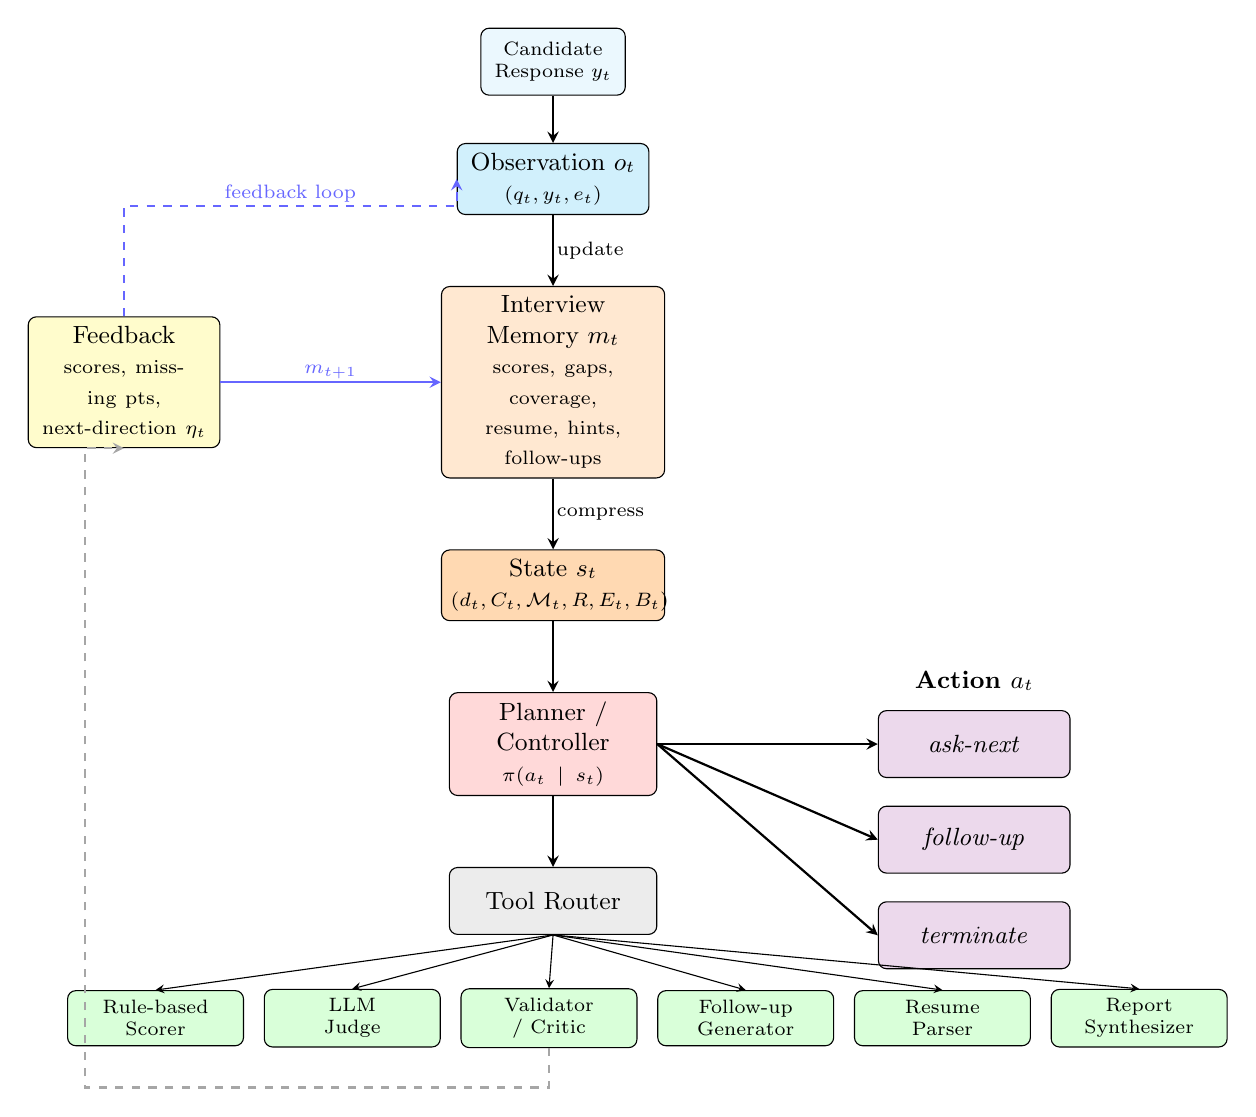
\begin{tikzpicture}[
    node distance=0.9cm and 1.2cm,
    block/.style={rectangle, draw, rounded corners=3pt, minimum height=0.85cm, text centered, font=\small},
    obs/.style={block, fill=cyan!18, text width=2.2cm},
    mem/.style={block, fill=orange!18, text width=2.6cm},
    ctrl/.style={block, fill=red!15, text width=2.4cm},
    tool/.style={block, fill=green!15, text width=2.0cm, minimum height=0.7cm, font=\scriptsize},
    act/.style={block, fill=violet!15, text width=2.2cm},
    fb/.style={block, fill=yellow!20, text width=2.2cm},
    arr/.style={->, >=stealth, thick},
    darr/.style={->, >=stealth, thick, dashed, gray!70},
    lbl/.style={font=\scriptsize, midway, fill=white, inner sep=1pt},
]

% === Row 1: Observation ===
\node[obs] (obs) {Observation $o_t$\\{\scriptsize $(q_t, y_t, e_t)$}};

% === Row 2: Memory ===
\node[mem, below=of obs] (mem) {Interview Memory $m_t$\\{\scriptsize scores, gaps, coverage,}\\{\scriptsize resume, hints, follow-ups}};

% === Row 3: State ===
\node[block, fill=orange!30, text width=2.6cm, below=of mem] (state) {State $s_t$\\{\scriptsize $(d_t, C_t, \mathcal{M}_t, R, E_t, B_t)$}};

% === Row 4: Controller ===
\node[ctrl, below=of state] (ctrl) {Planner / Controller\\{\scriptsize $\pi(a_t \mid s_t)$}};

% === Row 5: Tool Router ===
\node[block, fill=gray!15, text width=2.4cm, below=of ctrl, font=\small] (router) {Tool Router};

% === Tools (fanned below router) ===
\node[tool, below left=0.7cm and 2.6cm of router] (t1) {Rule-based\\Scorer};
\node[tool, right=0.25cm of t1] (t2) {LLM\\Judge};
\node[tool, right=0.25cm of t2] (t3) {Validator\\/ Critic};
\node[tool, right=0.25cm of t3] (t4) {Follow-up\\Generator};
\node[tool, right=0.25cm of t4] (t5) {Resume\\Parser};
\node[tool, right=0.25cm of t5] (t6) {Report\\Synthesizer};

% === Actions (right of controller) ===
\node[act, right=2.8cm of ctrl] (askn) {\textit{ask-next}};
\node[act, below=0.35cm of askn] (foll) {\textit{follow-up}};
\node[act, below=0.35cm of foll] (term) {\textit{terminate}};

% Action space label
\node[above=0.12cm of askn, font=\small\bfseries] {Action $a_t$};

% === Feedback (left of memory) ===
\node[fb, left=2.8cm of mem] (fb) {Feedback\\{\scriptsize scores, missing pts,}\\{\scriptsize next-direction $\eta_t$}};

% ===== Arrows =====
% Observation -> Memory
\draw[arr] (obs) -- node[lbl, right] {update} (mem);
% Memory -> State
\draw[arr] (mem) -- node[lbl, right] {compress} (state);
% State -> Controller
\draw[arr] (state) -- (ctrl);
% Controller -> Router
\draw[arr] (ctrl) -- (router);
% Controller -> Actions
\draw[arr] (ctrl.east) -- (askn.west);
\draw[arr] (ctrl.east) -- (foll.west);
\draw[arr] (ctrl.east) -- (term.west);

% Router -> Tools
\foreach \t in {t1,t2,t3,t4,t5,t6}
    \draw[arr, thin] (router.south) -- (\t.north);

% Feedback -> Memory (the loop)
\draw[arr, blue!60, thick] (fb) -- node[lbl, above] {$m_{t+1}$} (mem);

% Tools -> Feedback (close the loop)
\draw[darr] (t3.south) -- ++(0,-0.5) -| ([xshift=-0.5cm]fb.south) -- (fb.south);

% Candidate input to observation
\node[block, fill=cyan!8, text width=1.6cm, above=0.6cm of obs, font=\scriptsize] (cand) {Candidate\\Response $y_t$};
\draw[arr] (cand) -- (obs);

% Loop annotation
\draw[arr, blue!60, thick, dashed] (fb.north) -- ++(0,1.4) -| node[lbl, above, pos=0.25] {\scriptsize feedback loop} (obs.west);

\end{tikzpicture}


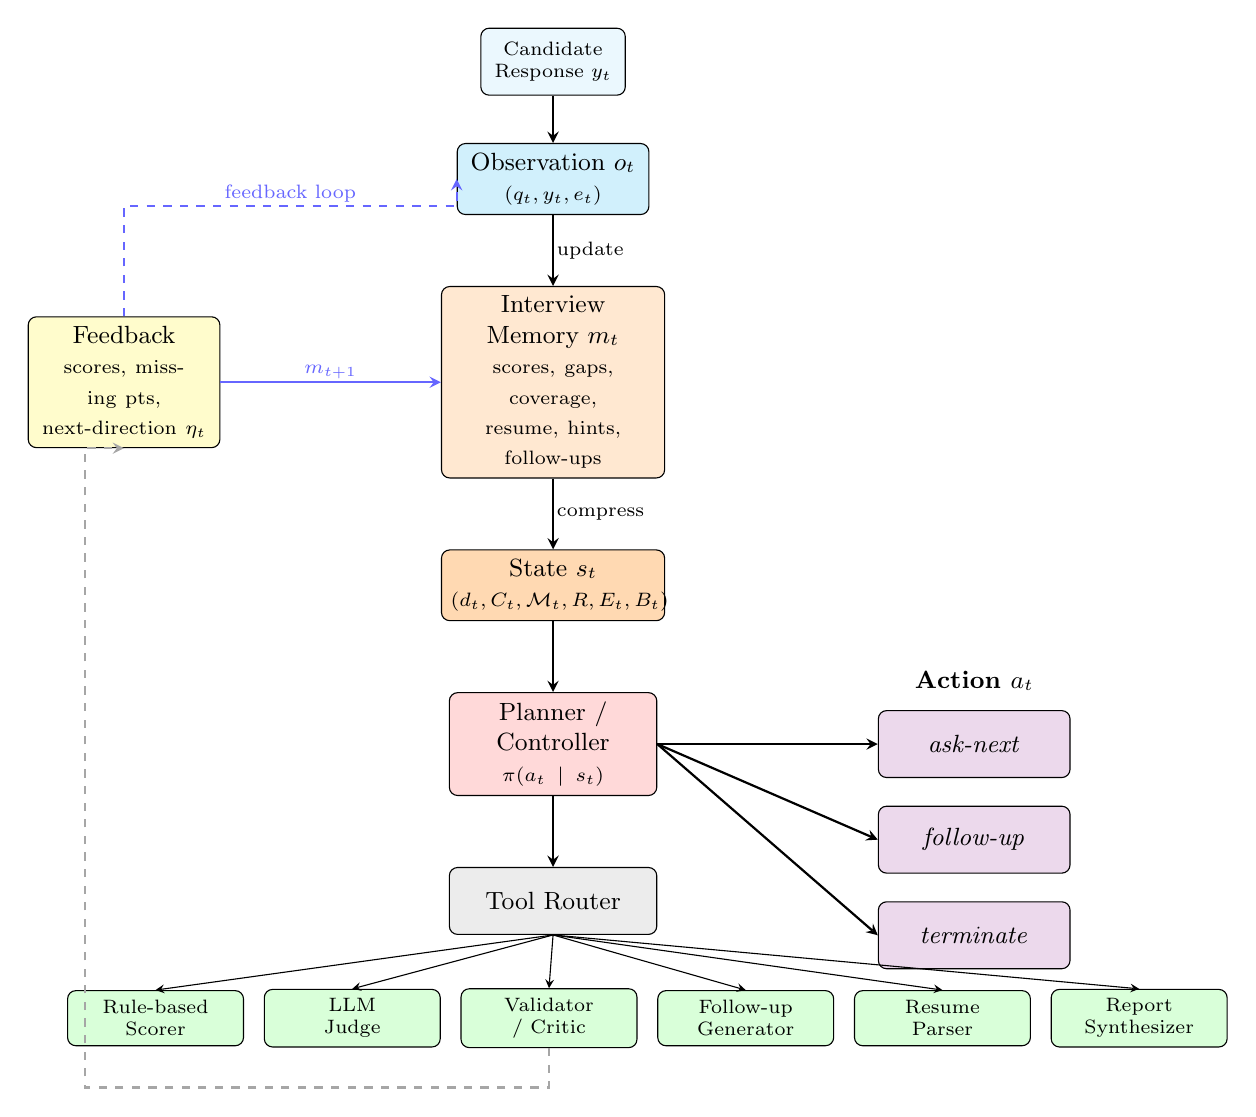
\begin{tikzpicture}[
    node distance=0.9cm and 1.2cm,
    block/.style={rectangle, draw, rounded corners=3pt, minimum height=0.85cm, text centered, font=\small},
    obs/.style={block, fill=cyan!18, text width=2.2cm},
    mem/.style={block, fill=orange!18, text width=2.6cm},
    ctrl/.style={block, fill=red!15, text width=2.4cm},
    tool/.style={block, fill=green!15, text width=2.0cm, minimum height=0.7cm, font=\scriptsize},
    act/.style={block, fill=violet!15, text width=2.2cm},
    fb/.style={block, fill=yellow!20, text width=2.2cm},
    arr/.style={->, >=stealth, thick},
    darr/.style={->, >=stealth, thick, dashed, gray!70},
    lbl/.style={font=\scriptsize, midway, fill=white, inner sep=1pt},
]

% === Row 1: Observation ===
\node[obs] (obs) {Observation $o_t$\\{\scriptsize $(q_t, y_t, e_t)$}};

% === Row 2: Memory ===
\node[mem, below=of obs] (mem) {Interview Memory $m_t$\\{\scriptsize scores, gaps, coverage,}\\{\scriptsize resume, hints, follow-ups}};

% === Row 3: State ===
\node[block, fill=orange!30, text width=2.6cm, below=of mem] (state) {State $s_t$\\{\scriptsize $(d_t, C_t, \mathcal{M}_t, R, E_t, B_t)$}};

% === Row 4: Controller ===
\node[ctrl, below=of state] (ctrl) {Planner / Controller\\{\scriptsize $\pi(a_t \mid s_t)$}};

% === Row 5: Tool Router ===
\node[block, fill=gray!15, text width=2.4cm, below=of ctrl, font=\small] (router) {Tool Router};

% === Tools (fanned below router) ===
\node[tool, below left=0.7cm and 2.6cm of router] (t1) {Rule-based\\Scorer};
\node[tool, right=0.25cm of t1] (t2) {LLM\\Judge};
\node[tool, right=0.25cm of t2] (t3) {Validator\\/ Critic};
\node[tool, right=0.25cm of t3] (t4) {Follow-up\\Generator};
\node[tool, right=0.25cm of t4] (t5) {Resume\\Parser};
\node[tool, right=0.25cm of t5] (t6) {Report\\Synthesizer};

% === Actions (right of controller) ===
\node[act, right=2.8cm of ctrl] (askn) {\textit{ask-next}};
\node[act, below=0.35cm of askn] (foll) {\textit{follow-up}};
\node[act, below=0.35cm of foll] (term) {\textit{terminate}};

% Action space label
\node[above=0.12cm of askn, font=\small\bfseries] {Action $a_t$};

% === Feedback (left of memory) ===
\node[fb, left=2.8cm of mem] (fb) {Feedback\\{\scriptsize scores, missing pts,}\\{\scriptsize next-direction $\eta_t$}};

% ===== Arrows =====
% Observation -> Memory
\draw[arr] (obs) -- node[lbl, right] {update} (mem);
% Memory -> State
\draw[arr] (mem) -- node[lbl, right] {compress} (state);
% State -> Controller
\draw[arr] (state) -- (ctrl);
% Controller -> Router
\draw[arr] (ctrl) -- (router);
% Controller -> Actions
\draw[arr] (ctrl.east) -- (askn.west);
\draw[arr] (ctrl.east) -- (foll.west);
\draw[arr] (ctrl.east) -- (term.west);

% Router -> Tools
\foreach \t in {t1,t2,t3,t4,t5,t6}
    \draw[arr, thin] (router.south) -- (\t.north);

% Feedback -> Memory (the loop)
\draw[arr, blue!60, thick] (fb) -- node[lbl, above] {$m_{t+1}$} (mem);

% Tools -> Feedback (close the loop)
\draw[darr] (t3.south) -- ++(0,-0.5) -| ([xshift=-0.5cm]fb.south) -- (fb.south);

% Candidate input to observation
\node[block, fill=cyan!8, text width=1.6cm, above=0.6cm of obs, font=\scriptsize] (cand) {Candidate\\Response $y_t$};
\draw[arr] (cand) -- (obs);

% Loop annotation
\draw[arr, blue!60, thick, dashed] (fb.north) -- ++(0,1.4) -| node[lbl, above, pos=0.25] {\scriptsize feedback loop} (obs.west);

\end{tikzpicture}
}
\caption{Overall memory-aware agentic interview framework. The system formulates adaptive interviewing as a closed-loop observation--memory--policy--action process, where a planner/controller invokes structured tools for question selection, judging, validation, follow-up generation, and report synthesis, while feedback signals are written back into persistent interview memory.}
\label{fig:agentic_framework}
\end{figure*}

% ================= Figure 2: Single-Turn Loop =================
\begin{figure*}[t]
\centering
\resizebox{\textwidth}{!}{% Single-Turn Decision Loop of the Interview Agent
% Use with: % Single-Turn Decision Loop of the Interview Agent
% Use with: % Single-Turn Decision Loop of the Interview Agent
% Use with: \input{figures/single_turn_loop.tex}

\begin{tikzpicture}[
    node distance=0.8cm and 1.5cm,
    step/.style={rectangle, draw, rounded corners=3pt, minimum height=0.75cm, text centered, font=\small, text width=2.8cm},
    decision/.style={diamond, draw, fill=red!10, aspect=2.2, inner sep=1pt, font=\small, text width=1.8cm, text centered},
    arr/.style={->, >=stealth, thick},
    lbl/.style={font=\scriptsize, fill=white, inner sep=1pt},
]

% === Left column: Input and Judging ===
\node[step, fill=cyan!15] (input) {Candidate response $y_t$};
\node[step, fill=green!12, below=of input] (rule) {Rule-based Judge\\{\scriptsize 5-dim scores $S_{\text{rule}}$}};
\node[decision, below=0.9cm of rule] (llmavail) {LLM\\avail?};
\node[step, fill=green!20, below left=0.9cm and 0.2cm of llmavail] (llm) {LLM Judge\\{\scriptsize scores + $\eta_t$}};
\node[decision, below=0.9cm of llm] (valid) {Valid?};

% === Middle column: Memory and State ===
\node[step, fill=orange!18, right=3.5cm of valid] (memup) {Update Memory $m_t$\\{\scriptsize append scores, gaps,}\\{\scriptsize coverage, hints}};
\node[step, fill=orange!28, below=of memup] (stateup) {Compute State $s_t$\\{\scriptsize $(d_t, C_t, \mathcal{M}_t, R, E_t, B_t)$}};

% === Right column: Controller Decisions ===
\node[decision, below=0.9cm of stateup] (termq) {Termi-\\nate?};
\node[decision, right=1.8cm of termq] (followq) {Follow\\up?};

% === Outcomes ===
\node[step, fill=violet!15, below=0.9cm of termq] (stop) {\textit{terminate}\\{\scriptsize generate report}};
\node[step, fill=violet!15, below=0.9cm of followq] (fu) {\textit{follow-up}\\{\scriptsize probe misconception}};
\node[step, fill=violet!15, right=1.8cm of followq] (next) {\textit{ask-next}\\{\scriptsize update $d_{t+1}$, select $q_{t+1}$}};

% === Merge / Fallback ===
\node[step, fill=yellow!15, below right=0.9cm and 0.2cm of llmavail] (fallback) {Fallback to\\$S_{\text{rule}}$};

% ===== Arrows =====
\draw[arr] (input) -- (rule);
\draw[arr] (rule) -- (llmavail);
\draw[arr] (llmavail) -- node[lbl, left] {yes} (llm);
\draw[arr] (llmavail) -- node[lbl, right] {no} (fallback);
\draw[arr] (llm) -- (valid);
\draw[arr] (valid.east) -- node[lbl, above] {yes} ++(1.5,0) |- (memup.west);
\draw[arr] (valid.south) -- node[lbl, left] {no} ++(0,-0.6) -| (fallback.south);
\draw[arr] (fallback.east) -| ([xshift=-0.4cm]memup.west) -- (memup.west);
\draw[arr] (memup) -- (stateup);
\draw[arr] (stateup) -- (termq);
\draw[arr] (termq) -- node[lbl, left] {yes} (stop);
\draw[arr] (termq) -- node[lbl, above] {no} (followq);
\draw[arr] (followq) -- node[lbl, left] {yes} (fu);
\draw[arr] (followq) -- node[lbl, above] {no} (next);

% Next turn arrow (loop back)
\draw[arr, blue!60, thick, dashed] (next.north) -- ++(0,1) -| node[lbl, above, pos=0.3] {\scriptsize next turn $t{+}1$} ([xshift=0.5cm]input.east) -- (input.east);
\draw[arr, blue!60, thick, dashed] (fu.west) -- ++(-0.8,0) |- node[lbl, left, pos=0.25] {} ([yshift=-0.15cm]input.south west) -- (input.south);

\end{tikzpicture}


\begin{tikzpicture}[
    node distance=0.8cm and 1.5cm,
    step/.style={rectangle, draw, rounded corners=3pt, minimum height=0.75cm, text centered, font=\small, text width=2.8cm},
    decision/.style={diamond, draw, fill=red!10, aspect=2.2, inner sep=1pt, font=\small, text width=1.8cm, text centered},
    arr/.style={->, >=stealth, thick},
    lbl/.style={font=\scriptsize, fill=white, inner sep=1pt},
]

% === Left column: Input and Judging ===
\node[step, fill=cyan!15] (input) {Candidate response $y_t$};
\node[step, fill=green!12, below=of input] (rule) {Rule-based Judge\\{\scriptsize 5-dim scores $S_{\text{rule}}$}};
\node[decision, below=0.9cm of rule] (llmavail) {LLM\\avail?};
\node[step, fill=green!20, below left=0.9cm and 0.2cm of llmavail] (llm) {LLM Judge\\{\scriptsize scores + $\eta_t$}};
\node[decision, below=0.9cm of llm] (valid) {Valid?};

% === Middle column: Memory and State ===
\node[step, fill=orange!18, right=3.5cm of valid] (memup) {Update Memory $m_t$\\{\scriptsize append scores, gaps,}\\{\scriptsize coverage, hints}};
\node[step, fill=orange!28, below=of memup] (stateup) {Compute State $s_t$\\{\scriptsize $(d_t, C_t, \mathcal{M}_t, R, E_t, B_t)$}};

% === Right column: Controller Decisions ===
\node[decision, below=0.9cm of stateup] (termq) {Termi-\\nate?};
\node[decision, right=1.8cm of termq] (followq) {Follow\\up?};

% === Outcomes ===
\node[step, fill=violet!15, below=0.9cm of termq] (stop) {\textit{terminate}\\{\scriptsize generate report}};
\node[step, fill=violet!15, below=0.9cm of followq] (fu) {\textit{follow-up}\\{\scriptsize probe misconception}};
\node[step, fill=violet!15, right=1.8cm of followq] (next) {\textit{ask-next}\\{\scriptsize update $d_{t+1}$, select $q_{t+1}$}};

% === Merge / Fallback ===
\node[step, fill=yellow!15, below right=0.9cm and 0.2cm of llmavail] (fallback) {Fallback to\\$S_{\text{rule}}$};

% ===== Arrows =====
\draw[arr] (input) -- (rule);
\draw[arr] (rule) -- (llmavail);
\draw[arr] (llmavail) -- node[lbl, left] {yes} (llm);
\draw[arr] (llmavail) -- node[lbl, right] {no} (fallback);
\draw[arr] (llm) -- (valid);
\draw[arr] (valid.east) -- node[lbl, above] {yes} ++(1.5,0) |- (memup.west);
\draw[arr] (valid.south) -- node[lbl, left] {no} ++(0,-0.6) -| (fallback.south);
\draw[arr] (fallback.east) -| ([xshift=-0.4cm]memup.west) -- (memup.west);
\draw[arr] (memup) -- (stateup);
\draw[arr] (stateup) -- (termq);
\draw[arr] (termq) -- node[lbl, left] {yes} (stop);
\draw[arr] (termq) -- node[lbl, above] {no} (followq);
\draw[arr] (followq) -- node[lbl, left] {yes} (fu);
\draw[arr] (followq) -- node[lbl, above] {no} (next);

% Next turn arrow (loop back)
\draw[arr, blue!60, thick, dashed] (next.north) -- ++(0,1) -| node[lbl, above, pos=0.3] {\scriptsize next turn $t{+}1$} ([xshift=0.5cm]input.east) -- (input.east);
\draw[arr, blue!60, thick, dashed] (fu.west) -- ++(-0.8,0) |- node[lbl, left, pos=0.25] {} ([yshift=-0.15cm]input.south west) -- (input.south);

\end{tikzpicture}


\begin{tikzpicture}[
    node distance=0.8cm and 1.5cm,
    step/.style={rectangle, draw, rounded corners=3pt, minimum height=0.75cm, text centered, font=\small, text width=2.8cm},
    decision/.style={diamond, draw, fill=red!10, aspect=2.2, inner sep=1pt, font=\small, text width=1.8cm, text centered},
    arr/.style={->, >=stealth, thick},
    lbl/.style={font=\scriptsize, fill=white, inner sep=1pt},
]

% === Left column: Input and Judging ===
\node[step, fill=cyan!15] (input) {Candidate response $y_t$};
\node[step, fill=green!12, below=of input] (rule) {Rule-based Judge\\{\scriptsize 5-dim scores $S_{\text{rule}}$}};
\node[decision, below=0.9cm of rule] (llmavail) {LLM\\avail?};
\node[step, fill=green!20, below left=0.9cm and 0.2cm of llmavail] (llm) {LLM Judge\\{\scriptsize scores + $\eta_t$}};
\node[decision, below=0.9cm of llm] (valid) {Valid?};

% === Middle column: Memory and State ===
\node[step, fill=orange!18, right=3.5cm of valid] (memup) {Update Memory $m_t$\\{\scriptsize append scores, gaps,}\\{\scriptsize coverage, hints}};
\node[step, fill=orange!28, below=of memup] (stateup) {Compute State $s_t$\\{\scriptsize $(d_t, C_t, \mathcal{M}_t, R, E_t, B_t)$}};

% === Right column: Controller Decisions ===
\node[decision, below=0.9cm of stateup] (termq) {Termi-\\nate?};
\node[decision, right=1.8cm of termq] (followq) {Follow\\up?};

% === Outcomes ===
\node[step, fill=violet!15, below=0.9cm of termq] (stop) {\textit{terminate}\\{\scriptsize generate report}};
\node[step, fill=violet!15, below=0.9cm of followq] (fu) {\textit{follow-up}\\{\scriptsize probe misconception}};
\node[step, fill=violet!15, right=1.8cm of followq] (next) {\textit{ask-next}\\{\scriptsize update $d_{t+1}$, select $q_{t+1}$}};

% === Merge / Fallback ===
\node[step, fill=yellow!15, below right=0.9cm and 0.2cm of llmavail] (fallback) {Fallback to\\$S_{\text{rule}}$};

% ===== Arrows =====
\draw[arr] (input) -- (rule);
\draw[arr] (rule) -- (llmavail);
\draw[arr] (llmavail) -- node[lbl, left] {yes} (llm);
\draw[arr] (llmavail) -- node[lbl, right] {no} (fallback);
\draw[arr] (llm) -- (valid);
\draw[arr] (valid.east) -- node[lbl, above] {yes} ++(1.5,0) |- (memup.west);
\draw[arr] (valid.south) -- node[lbl, left] {no} ++(0,-0.6) -| (fallback.south);
\draw[arr] (fallback.east) -| ([xshift=-0.4cm]memup.west) -- (memup.west);
\draw[arr] (memup) -- (stateup);
\draw[arr] (stateup) -- (termq);
\draw[arr] (termq) -- node[lbl, left] {yes} (stop);
\draw[arr] (termq) -- node[lbl, above] {no} (followq);
\draw[arr] (followq) -- node[lbl, left] {yes} (fu);
\draw[arr] (followq) -- node[lbl, above] {no} (next);

% Next turn arrow (loop back)
\draw[arr, blue!60, thick, dashed] (next.north) -- ++(0,1) -| node[lbl, above, pos=0.3] {\scriptsize next turn $t{+}1$} ([xshift=0.5cm]input.east) -- (input.east);
\draw[arr, blue!60, thick, dashed] (fu.west) -- ++(-0.8,0) |- node[lbl, left, pos=0.25] {} ([yshift=-0.15cm]input.south west) -- (input.south);

\end{tikzpicture}
}
\caption{Single-turn decision loop of the interview agent. A candidate response is routed through hybrid judging, validated, converted into structured feedback signals, written into memory/state, and then used to choose the next action among asking a new question, generating a targeted follow-up, or terminating the interview.}
\label{fig:single_turn_loop}
\end{figure*}

\subsection{Adaptive Control: Difficulty Update and Termination}
\label{sec:adaptive_control}

\noindent This subsection specifies the \emph{control} half of RQ1's joint adaptive policy: a state-aware policy for difficulty calibration and budget-constrained interview termination. The controller observes performance signals from interview memory and adjusts the difficulty trajectory to converge on the candidate's ability level within a limited question budget; Section~\ref{sec:selection} specifies the coupled \emph{selection} half operating on the same memory.

\subsubsection{Adaptive Round Bounds}

\noindent The termination engine computes adaptive bounds from the user-specified target round count $r_{\text{user}}$:
\begin{equation}
n_{\min} = \max\left(3, \lfloor r_{\text{user}} \cdot \rho_{\min} \rfloor\right), \quad
n_{\max} = \min\left(n_{\text{cap}}, \lfloor r_{\text{user}} \cdot \rho_{\max} \rfloor\right)
\end{equation}
where $\rho_{\min}$ (default 0.5) and $\rho_{\max}$ (default 1.2) are configurable ratios and $n_{\text{cap}}$ (default 20) is the absolute upper bound.

\subsubsection{Performance Aggregation from Memory}

\noindent The controller computes performance metrics from the score history $\mathcal{S}_t$ in interview memory:

\begin{equation}
\bar{s} = \frac{1}{t} \sum_{i=1}^{t} s_i, \quad
\bar{s}_w = \frac{1}{\min(w, t)} \sum_{i=\max(1, t-w+1)}^{t} s_i, \quad
\sigma = \sqrt{\frac{1}{t} \sum_{i=1}^{t} (s_i - \bar{s})^2}
\end{equation}

where $w$ (default 3) is the sliding window size. These metrics capture overall performance, recent performance trend, and score stability. The difficulty range $R_d = \max_i d_i - \min_i d_i$ and chapter coverage $C = |\{c_i\}|$ are computed from the difficulty trajectory $\mathcal{D}_t$ and coverage trace $\mathcal{C}_t$ in memory.

\subsubsection{Termination Conditions}

\noindent The controller evaluates four termination conditions in sequence, each conditioned on the current state $s_t$:

\textbf{Condition 1: Early termination (excellent performance).}
\begin{equation}
T_1 = \begin{cases}
\text{True} & \text{if } \bar{s} \geq 0.85 \land \bar{s}_w \geq 0.85 \land \sigma < 0.15 \\
\text{False} & \text{otherwise}
\end{cases}
\end{equation}

\textbf{Condition 2: Early termination (consistently poor performance).}
\begin{equation}
T_2 = \begin{cases}
\text{True} & \text{if } \bar{s} < 0.4 \land \bar{s}_w < 0.4 \\
\text{False} & \text{otherwise}
\end{cases}
\end{equation}

\textbf{Condition 3: Normal termination (sufficient coverage and stability).}
\begin{equation}
T_3 = \begin{cases}
\text{True} & \text{if } \sigma < 0.2 \land R_d \geq 2 \land C \geq 3 \land \bar{s}_w \geq 0.7 \\
\text{False} & \text{otherwise}
\end{cases}
\end{equation}

\textbf{Condition 4: Forced termination (budget exhausted).}
\begin{equation}
T_4 = \begin{cases}
\text{True} & \text{if } t \geq r_{\text{user}} \lor t \geq n_{\max} \\
\text{False} & \text{otherwise}
\end{cases}
\end{equation}

Early termination ($T_1$, $T_2$, $T_3$) applies only when $t \geq n_{\min}$. The final decision: $\text{Terminate} = T_1 \lor T_2 \lor T_3 \lor T_4$.

\subsubsection{Trend-Aware Difficulty Update}

\noindent The difficulty update rule uses the sliding-window average $\bar{s}_w$ and a trend term $T = s_t - s_{t-1}$. Two update strategies are supported, controlled by configuration:

\begin{algorithm}[h]
\caption{Adaptive Control: Difficulty Update and Termination}
\label{alg:rq1}
\begin{algorithmic}[1]
\STATE \textbf{Input:} state $s_t$; memory $m_t$ (scores $\mathcal{S}_t$, difficulties $\mathcal{D}_t$, coverage $\mathcal{C}_t$); window $w$; budget parameters $r_{\text{user}}$, $\rho_{\min}$, $\rho_{\max}$, $n_{\text{cap}}$
\STATE \textbf{Output:} updated difficulty $d_{t+1}$; termination flag; reason
\STATE Compute $n_{\min}$, $n_{\max}$ from budget parameters
\IF{$t \ge r_{\text{user}}$} \STATE \textbf{return} $(d_t, \text{terminate}, \text{``user cap''})$ \ENDIF
\IF{$t \ge n_{\max}$} \STATE \textbf{return} $(d_t, \text{terminate}, \text{``max rounds''})$ \ENDIF
\IF{$t < n_{\min}$} \STATE skip termination check \ENDIF
\STATE Compute $\bar{s}$, $\bar{s}_w$, $\sigma$, $R_d$, $C$ from memory $m_t$
\STATE Evaluate $T_1 \lor T_2 \lor T_3$; if any true, \textbf{return} terminate
\STATE Compute trend $T \leftarrow s_t - s_{t-1}$ (if $t \ge 2$, else $0$)
\STATE \textbf{If} strategy = \texttt{heuristic}: update $d_{t+1}$ by threshold rules on $\bar{s}_w$ and $T$
\STATE \textbf{Else if} strategy = \texttt{target\_score\_control}: update $d_{t+1}$ targeting score $\tau$ with proportional-derivative correction
\STATE \textbf{return} $(d_{t+1}, \text{continue})$
\end{algorithmic}
\end{algorithm}

The \emph{heuristic} strategy applies threshold-based rules: if $\bar{s}_w \geq 0.85$, increase difficulty; if $\bar{s}_w < 0.4$, decrease; otherwise adjust based on trend. The \emph{target-score control} strategy adjusts difficulty based on proportional error $(\bar{s}_w - \tau)$ and a trend term, where $\tau$ (default 0.70) is the target score, making the intended operating point explicit.

\subsection{State-Aware Question Selection}
\label{sec:selection}

\noindent The question selection mechanism completes RQ1's joint adaptive policy through a multi-objective, state-conditioned policy grounded in the same $s_t$ and memory traces as Section~\ref{sec:adaptive_control}. Conceptually, the next question is chosen to maximize a composite objective:

\begin{equation}
q_{t+1} = \arg\max_{q \in Q_t} \Bigl[\lambda_1 \cdot \text{Gap}(q) + \lambda_2 \cdot \text{ResumeMatch}(q) + \lambda_3 \cdot \text{CoverageGain}(q) + \lambda_4 \cdot \text{Info}(q) + \lambda_5 \cdot \text{Explore}(q) + \lambda_6 \cdot \text{NextDir}(q)\Bigr]
\label{eq:selection_objective}
\end{equation}

where $Q_t$ is the set of unasked questions at the current difficulty, and the terms capture gap targeting, resume alignment, coverage maximization, Fisher information, exploration bonus, and evaluator next-direction alignment respectively.

The current implementation approximates this objective through a priority system that operates on the state $s_t = (d_t, C_t, \mathcal{M}_t, R, E_t, B_t)$. When an LLM is available, the system first invokes an \emph{LLM-as-topic-planner}: it sends the complete interview state (chapters covered with scores, identified gaps, resume skills, available chapters) to the language model and asks it to reason about which topic to explore next. The LLM returns a suggested chapter with a rationale, which is validated against the available chapter set via fuzzy matching. This ``Priority 0'' mechanism enables strategic, context-aware topic planning that goes beyond the priority cascade. When the LLM is unavailable or its suggestion does not match available chapters, the system falls back to the priority cascade below:

\begin{algorithm}[h]
\caption{State-Aware Multi-Objective Question Selection}
\label{alg:rq2}
\begin{algorithmic}[1]
\STATE \textbf{Input:} question bank $Q$; asked set $A$; state $s_t$ (difficulty $d_t$, coverage $C_t$, missing concepts $\mathcal{M}_t$, resume $R$, evaluation $E_t$ with hint $\eta_t$)
\STATE \textbf{Output:} next question $q_{t+1}$
\STATE If $\eta_t \neq \emptyset$: augment $\mathcal{M}_t \leftarrow \mathcal{M}_t \cup \{\text{chapters matched from } \eta_t \text{ (fuzzy, $>60\%$)}\}$
\STATE Select target chapter $\hat{c}$ by priorities:
\STATE \quad P1 (Gap): match $\mathcal{M}_t$ to chapters (avoid recently used)
\STATE \quad P2 (Resume): match $R$ to chapters (avoid repeats)
\STATE \quad P3 (Coverage): sample from $C_t$ via weighted-random, Thompson sampling, or UCB
\STATE Candidate set $Q_c \leftarrow \{q \in Q : q.\text{chapter} \approx \hat{c},\, q.\text{difficulty} = d_t,\, q \notin A\}$
\IF{$Q_c = \emptyset$} \STATE relax chapter match, then difficulty \ENDIF
\IF{strategy = \texttt{personalized}}
    \STATE Estimate ability $\hat{\theta}$ from memory (Eq.~\ref{eq:ability})
    \STATE Score: $s(q) = I_{\text{Fisher}}(\hat{\theta}, q.d) \cdot w_{\text{UCB}}(q.\text{chapter}) \cdot w_{\text{pers}}(q.\text{chapter})$
    \STATE With probability $\epsilon$: \textbf{return} random from $Q_c$
    \STATE \textbf{return} $\arg\max_{q \in Q_c} s(q)$
\ELSE
    \STATE \textbf{return} uniform sample from $Q_c$
\ENDIF
\end{algorithmic}
\end{algorithm}

\subsubsection{Priority 1: Gap Targeting with Evaluator Feedback}

\noindent Priority one $P_1(\mathcal{M}_t)$ targets chapters corresponding to identified knowledge gaps. When the LLM evaluator provides a next-direction hint $\eta_t$ (e.g., ``explore concurrency in depth''), the system fuzzy-matches $\eta_t$ to track chapters (threshold 60\%) and augments the missing-concept set $\mathcal{M}_t$ before applying priorities. This creates an \emph{evaluation-to-selection feedback loop} that closes the gap between assessment and selection---a key instance of memory-driven action conditioning.

For each missing concept $m_i \in \mathcal{M}_t$:
\begin{equation}
P_1(\mathcal{M}_t) = \arg\max_{c \in C} \left\{ \text{similarity}(m_i, c) \mid \text{similarity}(m_i, c) > 0.7,\, c \notin \mathcal{C}_{t}[-2:] \right\}
\end{equation}

\subsubsection{Priority 2: Resume-Derived Personalization}

\noindent Priority two $P_2(R)$ matches parsed resume skills to chapters:
\begin{equation}
P_2(R) = \arg\max_{c \in C} \left\{ \text{similarity}(r_j, c) \mid r_j \in R,\, \text{similarity}(r_j, c) > 0.7,\, c \notin \mathcal{C}_{t}[-2:] \right\}
\end{equation}

\subsubsection{Priority 3: Coverage-Driven Exploration}

\noindent Priority three implements the coverage fallback. In the default configuration, it uses weighted random selection. Optionally, Thompson sampling (Beta-Bernoulli) provides an exploration--exploitation trade-off conditioned on the current difficulty level:
\begin{equation}
P(c_i) = \frac{w_i \cdot I(c_i \notin \mathcal{C}_t[-2:])}{\sum_{j} w_j \cdot I(c_j \notin \mathcal{C}_t[-2:])}
\end{equation}

\subsubsection{Personalized Mode: IRT-Inspired Ability Estimation}

\noindent When \texttt{selector\_strategy=personalized}, the system augments the multi-priority framework with IRT-inspired ability estimation and Fisher information maximization. The ability estimate uses a weighted average over recent history:

\begin{equation}
\hat{\theta} = \frac{\sum_{i=1}^{|\mathcal{H}_t|} w_i \cdot \text{clip}\left(d_i + (s_i - 0.5) \cdot 2, \; 1, \; 5\right)}{\sum_{i} w_i}, \quad w_i = i
\label{eq:ability}
\end{equation}

Fisher information proxy favors items whose difficulty matches the estimated ability:
\begin{equation}
I_{\text{Fisher}}(\hat{\theta}, b) = \frac{1}{1 + 0.5 \cdot |\hat{\theta} - b|}
\end{equation}

UCB-based chapter exploration balances under-sampled chapters with weak areas:
\begin{equation}
\text{UCB}(c) = \bar{s}_c + \eta \sqrt{\frac{\ln(N+1)}{n_c}}
\end{equation}

The final item score combines Fisher information, UCB, and personalization:
\begin{equation}
s(q) = I_{\text{Fisher}}(\hat{\theta}, q.d) \cdot \left(0.5 + 0.5 \cdot \min(\text{UCB}(q.\text{chapter}), 2)\right) \cdot w_{\text{pers}}(q.\text{chapter})
\end{equation}

With probability $\epsilon$ (default 0.15), the system selects a random item from $Q_c$ for exploration.

\subsection{Follow-up Planning}
\label{sec:followup}

\noindent Follow-up is a distinct agent action conditioned on the current state: the controller decides to probe deeper rather than moving to a new question. The follow-up decision is conditioned on:
\begin{itemize}
    \item Misconceptions identified in $\mathcal{M}_t$
    \item The most recent next-direction hint $\eta_t$
    \item The follow-up trace $\mathcal{F}_t$ (how many follow-ups this question has received)
    \item A per-question follow-up budget $k_{\max}$ (default 2)
\end{itemize}

\begin{algorithm}[h]
\caption{Follow-up Decision and Generation}
\label{alg:followup}
\begin{algorithmic}[1]
\STATE \textbf{Input:} state $s_t$; current question $q_t$; evaluation score $s_t$; missing points $M_t^{\text{new}}$; follow-up count $k$ for $q_t$
\STATE \textbf{Output:} follow-up decision (boolean); follow-up text $f$ (if applicable)
\IF{$k \geq k_{\max}$} \STATE \textbf{return} (False, $\bot$) \ENDIF
\IF{$s_t < 0.6 \land |M_t^{\text{new}}| > 0 \land \neg\text{similar\_followup}(q_t, M_t^{\text{new}}[0])$}
    \STATE \textbf{return} (True, $G(q_t, y_t, M_t^{\text{new}}, k)$)
\ENDIF
\IF{$0.6 \leq s_t < 0.7 \land |M_t^{\text{new}}| > 0 \land k < 1$}
    \STATE \textbf{return} (True, $G(q_t, y_t, M_t^{\text{new}}, k)$)
\ENDIF
\STATE \textbf{return} (False, $\bot$)
\end{algorithmic}
\end{algorithm}

The follow-up generator $G(q_t, y_t, M_t^{\text{new}}, k)$ produces a targeted probe. When an LLM is available, it uses a structured prompt including the question, candidate answer, evaluation feedback, and missing points. The prompt requests a short, targeted follow-up addressing the specific misconception. When the LLM is unavailable, the system falls back to template-based generation using the first missing point in predefined phrasings. The depth adapts to $k$: the first follow-up targets the knowledge gap concretely; the second may shift angle or ask for a practical scenario.

\subsection{Reliability-Constrained Hybrid Judging}
\label{sec:hybrid_judging}

\noindent The hybrid judging framework implements the \emph{online evaluation module}: routing between rule-based and LLM judges, validation, fallback, and optional multi-judge aggregation. It is not framed as a standalone contribution (C1--C4 foreground the joint policy, session-level report analysis, and learner-centered evaluation); rather, it supplies structured scores, missing concepts, and next-direction hints $\eta_t$ that close the loop into memory and selection. The framework operates as a tool invoked at each turn, producing structured evaluation output that is written back into interview memory.

\begin{algorithm}[h]
\caption{Reliability-Constrained Hybrid Judging with Routing and Fallback}
\label{alg:rq3}
\begin{algorithmic}[1]
\STATE \textbf{Input:} question $q$; reference answer $a^*$; candidate response $y$; LLM availability flag; judge count $J$ (\texttt{llm\_multi\_judge\_count})
\STATE \textbf{Output:} five-dimension scores + overall score; feedback; next-direction hint $\eta$; provenance
\STATE \textbf{Step 1 (Rule-based judge):} Compute deterministic scores $S_{\text{rule}}$ across five dimensions
\IF{LLM available}
    \STATE \textbf{Step 2 (LLM judge):} Query LLM with fixed rubric, structured schema, optional CoT (\texttt{llm\_use\_cot})
    \IF{$J > 1$}
        \STATE \textbf{Step 2b (Multi-judge):} Run $J$ independent LLM evaluations; aggregate scores by mean; merge missing points by frequency
    \ENDIF
    \STATE \textbf{Step 3 (Validator):} Check schema compliance, score range $[0,1]$, required fields
    \IF{validation passes}
        \STATE Combine $S_{\text{rule}}$ and $S_{\text{llm}}$; extract $\eta$; provenance $\leftarrow$ hybrid
\ELSE
        \STATE Fallback to $S_{\text{rule}}$; provenance $\leftarrow$ rule (validation failure)
\ENDIF
\ELSE
    \STATE provenance $\leftarrow$ rule (LLM unavailable)
\ENDIF
\STATE \textbf{return} scores, feedback, $\eta$, provenance
\end{algorithmic}
\end{algorithm}

% ================= Figure 3: Hybrid Judging =================
\begin{figure*}[t]
\centering
\resizebox{\textwidth}{!}{% Reliability-Constrained Hybrid Judging with Optional Multi-Judge Aggregation
% Use with: % Reliability-Constrained Hybrid Judging with Optional Multi-Judge Aggregation
% Use with: % Reliability-Constrained Hybrid Judging with Optional Multi-Judge Aggregation
% Use with: \input{figures/hybrid_judging.tex}

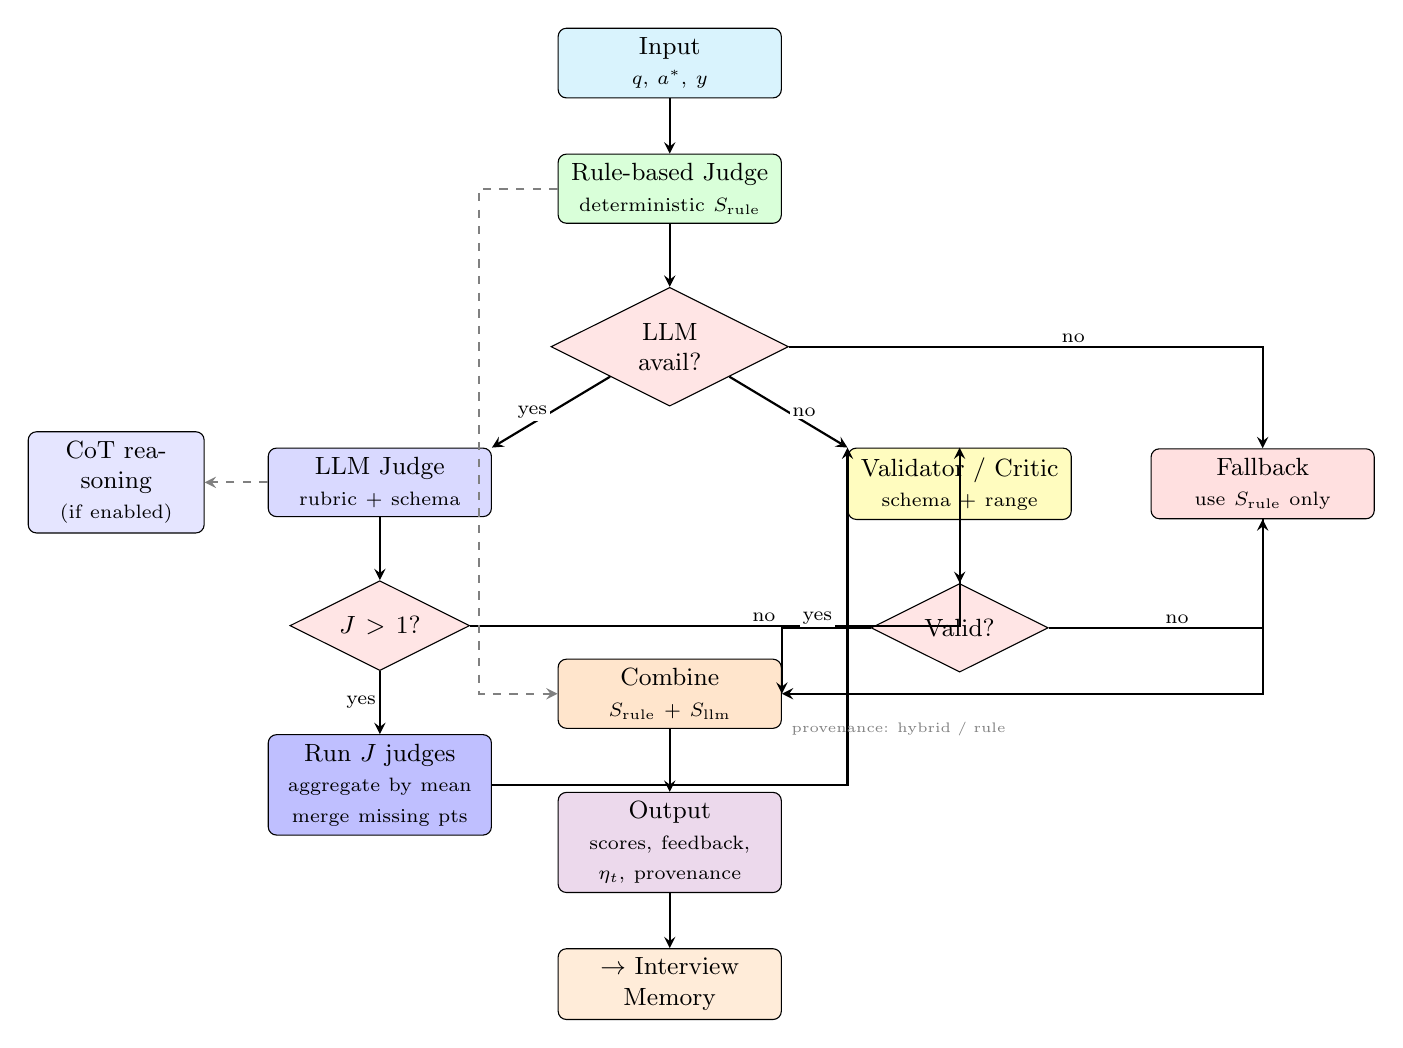
\begin{tikzpicture}[
    node distance=0.7cm and 1.0cm,
    block/.style={rectangle, draw, rounded corners=3pt, minimum height=0.7cm, text centered, font=\small, text width=2.6cm},
    decision/.style={diamond, draw, fill=red!10, aspect=2, inner sep=1pt, font=\small, text width=1.6cm, text centered},
    arr/.style={->, >=stealth, thick},
    lbl/.style={font=\scriptsize, fill=white, inner sep=1pt},
]

% === Input ===
\node[block, fill=cyan!15] (input) {Input\\{\scriptsize $q$, $a^*$, $y$}};

% === Rule-based Judge (always runs) ===
\node[block, fill=green!15, below=of input] (rule) {Rule-based Judge\\{\scriptsize deterministic $S_{\text{rule}}$}};

% === LLM availability check ===
\node[decision, below=0.8cm of rule] (llmcheck) {LLM\\avail?};

% === LLM Judge branch ===
\node[block, fill=blue!15, below left=0.9cm and 1.5cm of llmcheck] (llmj) {LLM Judge\\{\scriptsize rubric + schema}};

% === Multi-judge check ===
\node[decision, below=0.8cm of llmj] (multij) {$J > 1$?};

% === Multi-judge ===
\node[block, fill=blue!25, below=0.8cm of multij] (agg) {Run $J$ judges\\{\scriptsize aggregate by mean}\\{\scriptsize merge missing pts}};

% === CoT check ===
\node[block, fill=blue!10, left=0.8cm of llmj, text width=2.0cm] (cot) {CoT reasoning\\{\scriptsize (if enabled)}};

% === Validator ===
\node[block, fill=yellow!25, below right=0.9cm and 1.5cm of llmcheck] (val) {Validator / Critic\\{\scriptsize schema + range}};

% === Validation decision ===
\node[decision, below=0.8cm of val] (valcheck) {Valid?};

% === Combine ===
\node[block, fill=orange!20, below=3.2cm of llmcheck] (combine) {Combine\\{\scriptsize $S_{\text{rule}}$ + $S_{\text{llm}}$}};

% === Fallback ===
\node[block, fill=red!12, right=1.0cm of val] (fallback) {Fallback\\{\scriptsize use $S_{\text{rule}}$ only}};

% === Output ===
\node[block, fill=violet!15, below=0.8cm of combine] (output) {Output\\{\scriptsize scores, feedback,}\\{\scriptsize $\eta_t$, provenance}};

% === To Memory ===
\node[block, fill=orange!15, below=0.7cm of output, text width=2.6cm] (tomem) {$\rightarrow$ Interview Memory};

% ===== Arrows =====
\draw[arr] (input) -- (rule);
\draw[arr] (rule) -- (llmcheck);

% LLM available -> LLM Judge
\draw[arr] (llmcheck.south west) -- node[lbl, left] {yes} (llmj.north east);
% LLM unavailable -> Fallback via validator area
\draw[arr] (llmcheck.south east) -- node[lbl, right] {no} (val.north west);
% but actually if LLM unavailable, go straight to fallback
\draw[arr] (llmcheck.east) -| node[lbl, above, pos=0.3] {no} (fallback.north);

% CoT
\draw[arr, dashed, gray] (llmj.west) -- (cot.east);

% LLM Judge -> Multi-judge check
\draw[arr] (llmj) -- (multij);

% Multi-judge yes -> aggregate
\draw[arr] (multij) -- node[lbl, left] {yes} (agg);
% Multi-judge no -> validator
\draw[arr] (multij.east) -| node[lbl, above, pos=0.3] {no} (val.north);

% Aggregate -> validator
\draw[arr] (agg.east) -| (val.north west);

% Validator -> validation check
\draw[arr] (val) -- (valcheck);

% Valid -> combine
\draw[arr] (valcheck.west) -| node[lbl, above, pos=0.3] {yes} (combine.east);
% Invalid -> fallback
\draw[arr] (valcheck.east) -| node[lbl, above, pos=0.3] {no} (fallback.south);

% Fallback -> combine (with rule-only provenance)
\draw[arr] (fallback.south) |- (combine.east);

% Rule also feeds combine directly
\draw[arr, dashed, gray] (rule.west) -| ([xshift=-1cm]combine.west) -- (combine.west);

% Combine -> Output
\draw[arr] (combine) -- (output);
% Output -> Memory
\draw[arr] (output) -- (tomem);

% Provenance labels
\node[font=\tiny, gray, right] at (combine.south east) {provenance: hybrid / rule};

\end{tikzpicture}


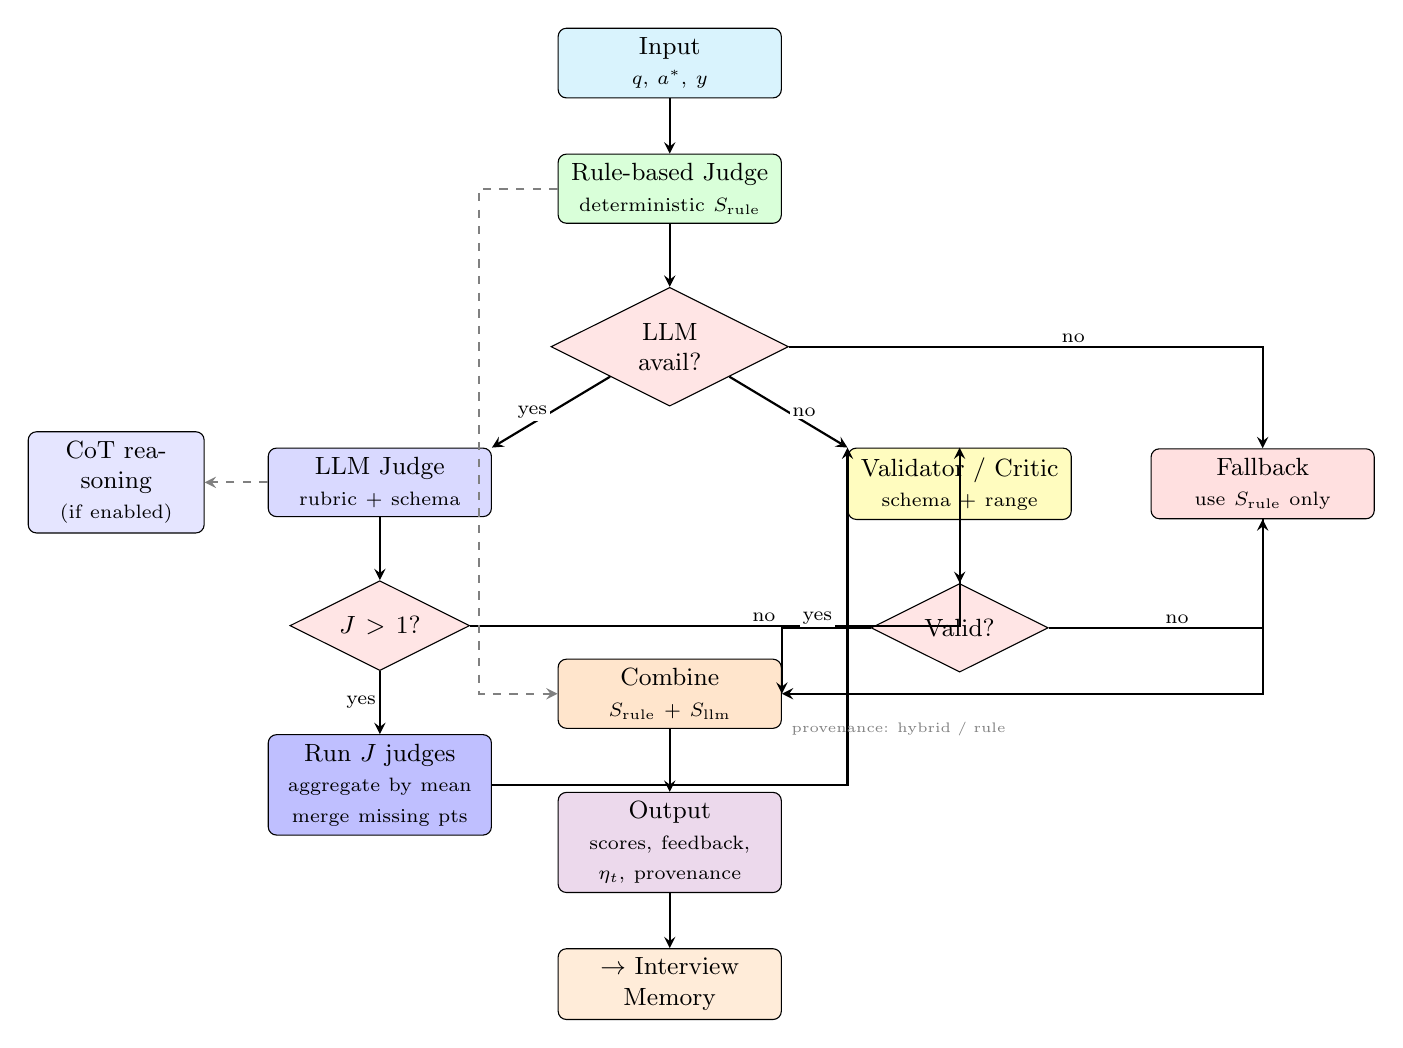
\begin{tikzpicture}[
    node distance=0.7cm and 1.0cm,
    block/.style={rectangle, draw, rounded corners=3pt, minimum height=0.7cm, text centered, font=\small, text width=2.6cm},
    decision/.style={diamond, draw, fill=red!10, aspect=2, inner sep=1pt, font=\small, text width=1.6cm, text centered},
    arr/.style={->, >=stealth, thick},
    lbl/.style={font=\scriptsize, fill=white, inner sep=1pt},
]

% === Input ===
\node[block, fill=cyan!15] (input) {Input\\{\scriptsize $q$, $a^*$, $y$}};

% === Rule-based Judge (always runs) ===
\node[block, fill=green!15, below=of input] (rule) {Rule-based Judge\\{\scriptsize deterministic $S_{\text{rule}}$}};

% === LLM availability check ===
\node[decision, below=0.8cm of rule] (llmcheck) {LLM\\avail?};

% === LLM Judge branch ===
\node[block, fill=blue!15, below left=0.9cm and 1.5cm of llmcheck] (llmj) {LLM Judge\\{\scriptsize rubric + schema}};

% === Multi-judge check ===
\node[decision, below=0.8cm of llmj] (multij) {$J > 1$?};

% === Multi-judge ===
\node[block, fill=blue!25, below=0.8cm of multij] (agg) {Run $J$ judges\\{\scriptsize aggregate by mean}\\{\scriptsize merge missing pts}};

% === CoT check ===
\node[block, fill=blue!10, left=0.8cm of llmj, text width=2.0cm] (cot) {CoT reasoning\\{\scriptsize (if enabled)}};

% === Validator ===
\node[block, fill=yellow!25, below right=0.9cm and 1.5cm of llmcheck] (val) {Validator / Critic\\{\scriptsize schema + range}};

% === Validation decision ===
\node[decision, below=0.8cm of val] (valcheck) {Valid?};

% === Combine ===
\node[block, fill=orange!20, below=3.2cm of llmcheck] (combine) {Combine\\{\scriptsize $S_{\text{rule}}$ + $S_{\text{llm}}$}};

% === Fallback ===
\node[block, fill=red!12, right=1.0cm of val] (fallback) {Fallback\\{\scriptsize use $S_{\text{rule}}$ only}};

% === Output ===
\node[block, fill=violet!15, below=0.8cm of combine] (output) {Output\\{\scriptsize scores, feedback,}\\{\scriptsize $\eta_t$, provenance}};

% === To Memory ===
\node[block, fill=orange!15, below=0.7cm of output, text width=2.6cm] (tomem) {$\rightarrow$ Interview Memory};

% ===== Arrows =====
\draw[arr] (input) -- (rule);
\draw[arr] (rule) -- (llmcheck);

% LLM available -> LLM Judge
\draw[arr] (llmcheck.south west) -- node[lbl, left] {yes} (llmj.north east);
% LLM unavailable -> Fallback via validator area
\draw[arr] (llmcheck.south east) -- node[lbl, right] {no} (val.north west);
% but actually if LLM unavailable, go straight to fallback
\draw[arr] (llmcheck.east) -| node[lbl, above, pos=0.3] {no} (fallback.north);

% CoT
\draw[arr, dashed, gray] (llmj.west) -- (cot.east);

% LLM Judge -> Multi-judge check
\draw[arr] (llmj) -- (multij);

% Multi-judge yes -> aggregate
\draw[arr] (multij) -- node[lbl, left] {yes} (agg);
% Multi-judge no -> validator
\draw[arr] (multij.east) -| node[lbl, above, pos=0.3] {no} (val.north);

% Aggregate -> validator
\draw[arr] (agg.east) -| (val.north west);

% Validator -> validation check
\draw[arr] (val) -- (valcheck);

% Valid -> combine
\draw[arr] (valcheck.west) -| node[lbl, above, pos=0.3] {yes} (combine.east);
% Invalid -> fallback
\draw[arr] (valcheck.east) -| node[lbl, above, pos=0.3] {no} (fallback.south);

% Fallback -> combine (with rule-only provenance)
\draw[arr] (fallback.south) |- (combine.east);

% Rule also feeds combine directly
\draw[arr, dashed, gray] (rule.west) -| ([xshift=-1cm]combine.west) -- (combine.west);

% Combine -> Output
\draw[arr] (combine) -- (output);
% Output -> Memory
\draw[arr] (output) -- (tomem);

% Provenance labels
\node[font=\tiny, gray, right] at (combine.south east) {provenance: hybrid / rule};

\end{tikzpicture}


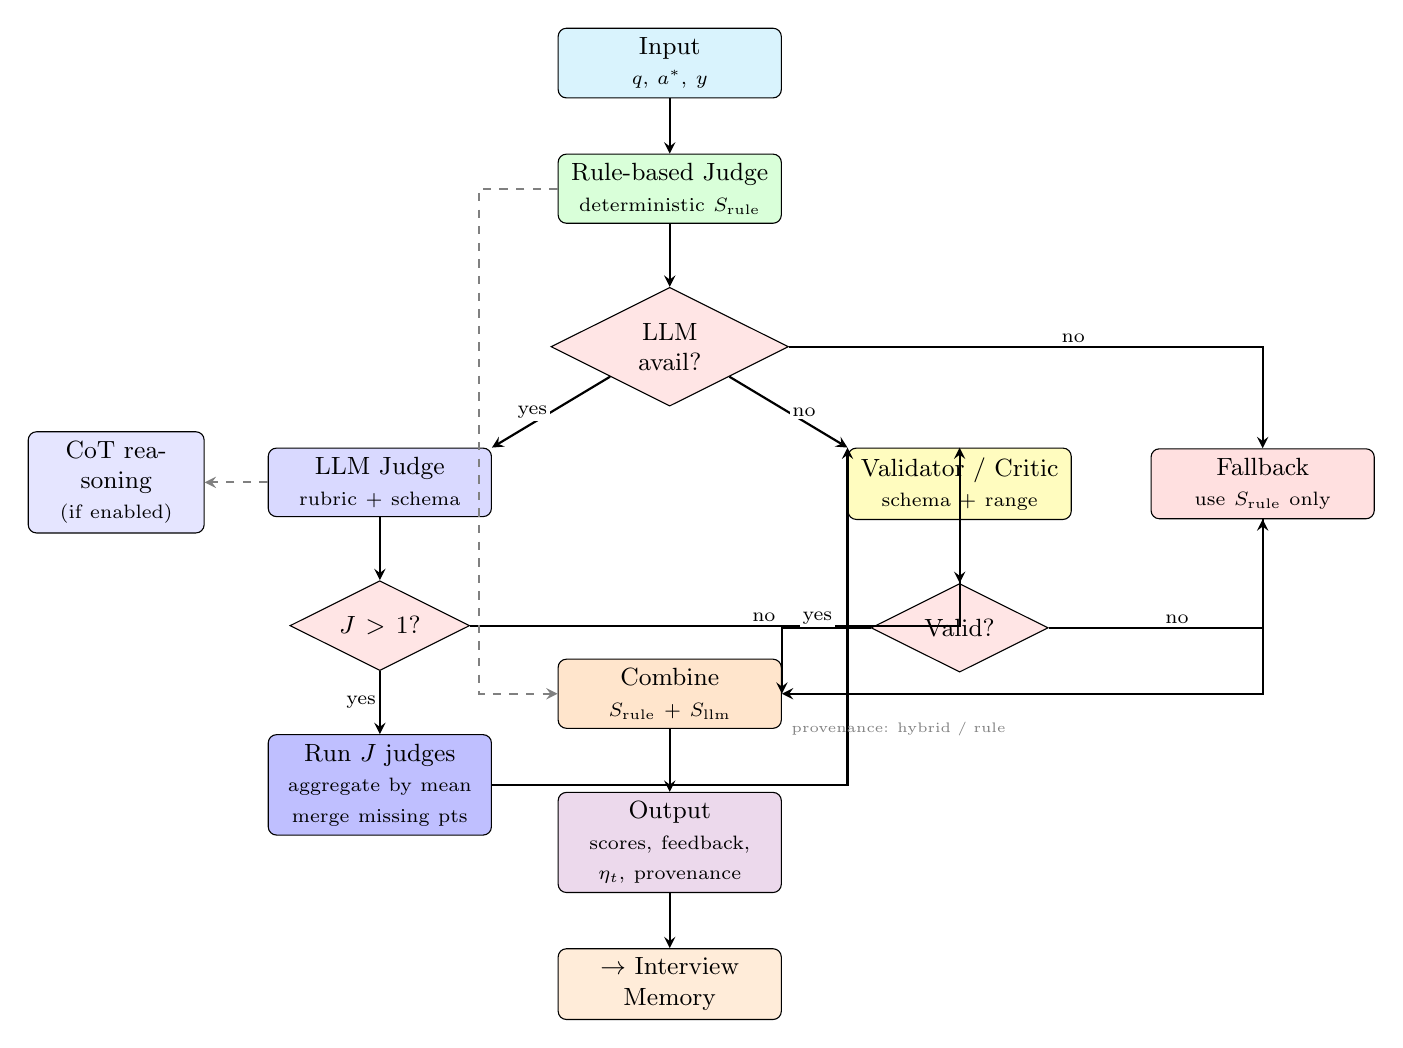
\begin{tikzpicture}[
    node distance=0.7cm and 1.0cm,
    block/.style={rectangle, draw, rounded corners=3pt, minimum height=0.7cm, text centered, font=\small, text width=2.6cm},
    decision/.style={diamond, draw, fill=red!10, aspect=2, inner sep=1pt, font=\small, text width=1.6cm, text centered},
    arr/.style={->, >=stealth, thick},
    lbl/.style={font=\scriptsize, fill=white, inner sep=1pt},
]

% === Input ===
\node[block, fill=cyan!15] (input) {Input\\{\scriptsize $q$, $a^*$, $y$}};

% === Rule-based Judge (always runs) ===
\node[block, fill=green!15, below=of input] (rule) {Rule-based Judge\\{\scriptsize deterministic $S_{\text{rule}}$}};

% === LLM availability check ===
\node[decision, below=0.8cm of rule] (llmcheck) {LLM\\avail?};

% === LLM Judge branch ===
\node[block, fill=blue!15, below left=0.9cm and 1.5cm of llmcheck] (llmj) {LLM Judge\\{\scriptsize rubric + schema}};

% === Multi-judge check ===
\node[decision, below=0.8cm of llmj] (multij) {$J > 1$?};

% === Multi-judge ===
\node[block, fill=blue!25, below=0.8cm of multij] (agg) {Run $J$ judges\\{\scriptsize aggregate by mean}\\{\scriptsize merge missing pts}};

% === CoT check ===
\node[block, fill=blue!10, left=0.8cm of llmj, text width=2.0cm] (cot) {CoT reasoning\\{\scriptsize (if enabled)}};

% === Validator ===
\node[block, fill=yellow!25, below right=0.9cm and 1.5cm of llmcheck] (val) {Validator / Critic\\{\scriptsize schema + range}};

% === Validation decision ===
\node[decision, below=0.8cm of val] (valcheck) {Valid?};

% === Combine ===
\node[block, fill=orange!20, below=3.2cm of llmcheck] (combine) {Combine\\{\scriptsize $S_{\text{rule}}$ + $S_{\text{llm}}$}};

% === Fallback ===
\node[block, fill=red!12, right=1.0cm of val] (fallback) {Fallback\\{\scriptsize use $S_{\text{rule}}$ only}};

% === Output ===
\node[block, fill=violet!15, below=0.8cm of combine] (output) {Output\\{\scriptsize scores, feedback,}\\{\scriptsize $\eta_t$, provenance}};

% === To Memory ===
\node[block, fill=orange!15, below=0.7cm of output, text width=2.6cm] (tomem) {$\rightarrow$ Interview Memory};

% ===== Arrows =====
\draw[arr] (input) -- (rule);
\draw[arr] (rule) -- (llmcheck);

% LLM available -> LLM Judge
\draw[arr] (llmcheck.south west) -- node[lbl, left] {yes} (llmj.north east);
% LLM unavailable -> Fallback via validator area
\draw[arr] (llmcheck.south east) -- node[lbl, right] {no} (val.north west);
% but actually if LLM unavailable, go straight to fallback
\draw[arr] (llmcheck.east) -| node[lbl, above, pos=0.3] {no} (fallback.north);

% CoT
\draw[arr, dashed, gray] (llmj.west) -- (cot.east);

% LLM Judge -> Multi-judge check
\draw[arr] (llmj) -- (multij);

% Multi-judge yes -> aggregate
\draw[arr] (multij) -- node[lbl, left] {yes} (agg);
% Multi-judge no -> validator
\draw[arr] (multij.east) -| node[lbl, above, pos=0.3] {no} (val.north);

% Aggregate -> validator
\draw[arr] (agg.east) -| (val.north west);

% Validator -> validation check
\draw[arr] (val) -- (valcheck);

% Valid -> combine
\draw[arr] (valcheck.west) -| node[lbl, above, pos=0.3] {yes} (combine.east);
% Invalid -> fallback
\draw[arr] (valcheck.east) -| node[lbl, above, pos=0.3] {no} (fallback.south);

% Fallback -> combine (with rule-only provenance)
\draw[arr] (fallback.south) |- (combine.east);

% Rule also feeds combine directly
\draw[arr, dashed, gray] (rule.west) -| ([xshift=-1cm]combine.west) -- (combine.west);

% Combine -> Output
\draw[arr] (combine) -- (output);
% Output -> Memory
\draw[arr] (output) -- (tomem);

% Provenance labels
\node[font=\tiny, gray, right] at (combine.south east) {provenance: hybrid / rule};

\end{tikzpicture}
}
\caption{Reliability-constrained hybrid judging with optional multi-judge aggregation. The system conditionally invokes rule-based or LLM-based judging, validates outputs, aggregates multiple judges when enabled, and automatically falls back to deterministic scoring when LLM outputs fail validation or external services are unavailable.}
\label{fig:hybrid_judging}
\end{figure*}

\subsubsection{Rule-Based Judge}

\noindent The rule-based judge computes scores across five dimensions. Correctness combines keyword coverage with text similarity:
\begin{equation}
C = 0.6 \cdot C_{\text{coverage}} + 0.4 \cdot C_{\text{similarity}}
\end{equation}
Depth assesses how thoroughly key points are addressed. Clarity evaluates answer structure through pattern matching. Practicality identifies examples and real-world applications. Tradeoff analysis detects discussion of advantages, disadvantages, and comparisons. The overall score combines dimensions with weights: correctness 30\%, depth 25\%, clarity 20\%, practicality 15\%, tradeoffs 10\%.

\subsubsection{LLM Judge with Validation}

\noindent When LLM enhancement is available (GLM-4.7-Flash via ZhipuAI API), the system queries the LLM with the question, reference answer, and candidate response using a structured evaluation rubric. The LLM output includes five-dimensional scores, feedback, and a \texttt{next\_direction} field that is passed to the selection policy as $\eta_t$. Two configurable variants are implemented: (i)~\texttt{llm\_use\_cot}, which requests concise structured reasoning for interpretability; and (ii)~\texttt{llm\_multi\_judge\_count}, which runs $J$ independent LLM judges and aggregates scores by mean with frequency-based merge of missing points.

\subsubsection{Validator / Critic}

\noindent The validator checks LLM output for schema compliance (all required fields present), score range validity ($[0,1]$ per dimension), and structural integrity. If validation fails, the system automatically falls back to rule-based scores with provenance recorded as ``rule (validation failure).'' This mechanism ensures that malformed LLM outputs never propagate into interview memory.

\subsubsection{Automatic Fallback Router}

\noindent The fallback router handles three failure modes: (i)~LLM service unavailable (API timeout, network error), (ii)~LLM output fails validation, and (iii)~LLM output is structurally valid but scores are out of expected range. In all cases, the system seamlessly transitions to rule-based evaluation, maintaining continuous operation and evaluation quality.

\subsection{Tool-Augmented Architecture}
\label{sec:tools}

\noindent The interview agent invokes specialized tools through a tool router. Each tool is a self-contained module with defined input/output interfaces and graceful degradation behavior. Table~\ref{tab:tools} summarizes the tool inventory.

\begin{table}[H]
\centering
\caption{Tool inventory of the interview agent. Each tool is invoked by the controller through the tool router.}
\label{tab:tools}
\footnotesize
\begin{tabularx}{\textwidth}{l Y Y}
\toprule
\textbf{Tool} & \textbf{Function} & \textbf{Fallback} \\
\midrule
Rule-based scorer & Deterministic five-dimensional scoring & Always available \\
LLM judge & Nuanced evaluation with next-direction hints & $\rightarrow$ Rule-based scorer \\
Validator / critic & Schema and range checking of judge output & Reject and fall back \\
Follow-up generator & Misconception-aware probe generation & $\rightarrow$ Template-based \\
Resume parser & Extract structured skills/experience from PDF/DOCX & Proceed without personalization \\
Speech analyzer & Communication metrics (fluency, rate, nervousness) & $\rightarrow$ Text heuristics \\
Expression analyzer & Facial emotion analysis (nervousness, confidence) & Return None; proceed without \\
Report synthesizer & Multi-step agentic LLM report with deep analysis & $\rightarrow$ Rule-based report \\
LLM topic planner & Reason about next chapter based on full interview state & $\rightarrow$ Priority cascade \\
\bottomrule
\end{tabularx}
\end{table}

\noindent \textbf{LLM topic planner (innovation).} When available, the controller invokes the language model as a \emph{strategic topic planner}: the full interview state (chapters covered with scores, identified gaps, resume skills, remaining budget) is sent to the LLM, which returns a suggested chapter and reasoning. This enables context-aware, strategic topic selection that goes beyond rule-based priority cascades, while the suggestion is validated against the question bank via fuzzy matching before use.

\noindent \textbf{Resume parser.} Extracts structured information from PDF, DOCX, and image files. For images, the system uses an LLM vision model for OCR when available, with fallback to PyMuPDF. Education, experience, projects, and skills are structured into JSON. Fuzzy matching (70\% threshold) enables robust skill-to-chapter alignment for the selection policy.

\noindent \textbf{Speech analyzer.} Processes audio responses to extract communication metrics. Fluency assessment uses a weighted combination:
\begin{equation}
F = 0.3 \cdot S_{\text{rate}} + 0.3 \cdot S_{\text{pause-freq}} + 0.2 \cdot S_{\text{pause-dur}} + 0.2 \cdot S_{\text{correction}}
\end{equation}
Speech-derived signals are treated as auxiliary features (not primary decision criteria) and reported descriptively.

\noindent \textbf{Expression analyzer.} Uses DeepFace \cite{serengil2020deepface} for emotion detection from video frames sampled during the interview. Maps seven basic emotions to interview-relevant metrics: nervousness, confidence, and engagement. When DeepFace is unavailable or no face is detected, the module returns None---graceful degradation consistent with the tool-augmented design.

\noindent \textbf{Report synthesizer (multi-step agentic).}\label{sec:report_pipeline} Report generation (RQ2) decomposes the \emph{entire session} into analyzable units before multi-step reasoning. \textbf{Inputs aggregated from the datastore} include: per-turn evaluations (five-dimensional scores, overall score, missing concepts, feedback), asked questions (chapter, difficulty, stem text), optional resume skills, and auxiliary modality summaries (speech/expression) when available. \textbf{Compression} builds a compact linear digest: up to 15 recent questions are rendered as one line each (chapter, truncated stem, score, missing points), prepended with session-level scalars---track, round count, mean dimension scores, difficulty trajectory, chapter trajectory, and resume skills---forming a shared \texttt{base\_context} string for all LLM steps (see implementation: sequential calls with independent JSON/text parsing and fallbacks).

\begin{table}[H]
\centering
\caption{Session trace decomposition for report analysis (RQ2). Granularity progresses from global signals to interpretable subscores and narrative outputs.}
\label{tab:report_decomposition}
\footnotesize
\begin{tabularx}{\textwidth}{l Y}
\toprule
\textbf{Layer} & \textbf{Content and role} \\
\midrule
Session & Track, rounds, aggregate means, difficulty/chapter trajectories, resume snapshot \\
Per-question & Stem (truncated), chapter, difficulty, scores, missing concepts for that turn \\
Dimension-level & Five rubric dimensions aggregated; per-dimension text via structured JSON in Step~2 \\
Diagnostic & Union of missing knowledge; root-cause narrative (not mere list) in Step~3 \\
Metacognitive & Strategy trace: how difficulty and chapters evolved and why (Step~5) \\
\bottomrule
\end{tabularx}
\end{table}

\noindent Table~\ref{tab:report_decomposition} summarizes the hierarchy; Table~\ref{tab:report_steps} lists the five LLM analysis steps (each with rule-based or empty fallback). The pipeline is \emph{sequential} rather than a single monolithic prompt: later steps consume the same compressed trace but apply different analytic lenses---summative (1), attributive (2), diagnostic (3), prescriptive (4), and transparency-oriented (5)---aligning with formative-feedback and explainability goals discussed in related work on multi-step educational NLP \cite{wei2022chain,llm_formative2025}.

\begin{table}[H]
\centering
\caption{Five-step session-level report analysis pipeline (shared compressed context; independent fallbacks).}
\label{tab:report_steps}
\footnotesize
\begin{tabularx}{\textwidth}{c Y Y}
\toprule
\textbf{Step} & \textbf{Analytic goal} & \textbf{Output shape} \\
\midrule
1 & Personalized narrative assessment grounded in specific answers & Short paragraph \\
2 & Per-dimension attribution tied to concrete items & JSON (five fields) \\
3 & Knowledge-gap root causes and links between gaps & Short paragraph \\
4 & Actionable learning plan items & Line-separated list \\
5 & Interview strategy transparency (difficulty/chapter logic) & Short paragraph \\
\bottomrule
\end{tabularx}
\end{table}

%% ============================================================
%%  SECTION 4: IMPLEMENTATION
%% ============================================================
\section{Implementation}
\label{sec:implementation}

\noindent This section provides implementation details. We emphasize that the agentic formulation in Section~\ref{sec:method} is compatible with the current modular implementation---the observation--memory--policy--action loop is realized through the existing service architecture without requiring a system rewrite.

\subsection{System Overview}

\noindent The system implements a three-layer architecture: a presentation layer (Streamlit), a business logic layer (Python services), and a data persistence layer (SQLAlchemy with SQLite/MySQL). The agentic loop maps onto this architecture as follows: the presentation layer handles observation capture (candidate responses, audio, video); the business logic layer implements the controller, tool router, and all tools; and the data layer persists interview memory across turns.

Table~\ref{tab:algorithm_parameters} presents key parameters governing the controller, selection policy, and hybrid judging.

\begin{table}[H]
\centering
\caption{Key algorithm parameters and default values. Thresholds (0.85, 0.4, 0.15) are tuning heuristics. Sensitivity analysis in Section~\ref{sec:results_rq1}.}
\label{tab:algorithm_parameters}
\footnotesize
\setlength{\tabcolsep}{4pt}
\begin{tabularx}{\textwidth}{l c Y c}
\toprule
\textbf{Parameter} & \textbf{Default} & \textbf{Description} & \textbf{Tuning} \\
\midrule
Window Size & 3 & Sliding window for difficulty update & Fixed \\
User Rounds ($r_{\text{user}}$) & 10 & User-specified target round count (hard cap) & Fixed \\
Min Rounds Ratio ($\rho_{\min}$) & 0.5 & $n_{\min} = \max(3, r_{\text{user}} \cdot \rho_{\min})$ & Fixed \\
Max Rounds Ratio ($\rho_{\max}$) & 1.2 & $n_{\max} = \min(20, r_{\text{user}} \cdot \rho_{\max})$ & Fixed \\
Max Rounds Cap ($n_{\text{cap}}$) & 20 & Absolute upper bound on rounds & Fixed \\
Follow-up Limit & 2 & Maximum follow-ups per question & Fixed \\
Similarity Threshold & 70\% & Fuzzy matching threshold for chapters & Heuristic \\
Excellent Score & 0.85 & Threshold for excellent performance & Heuristic \\
Poor Score & 0.4 & Threshold for poor performance & Heuristic \\
Stability Threshold & 0.15 & Standard deviation threshold for stability & Heuristic \\
Selector Strategy & personalized & Selection policy: \texttt{weighted\_random}, \texttt{thompson\_sampling}, or \texttt{personalized} & Configurable \\
LLM CoT Toggle & false & Enable structured reasoning in judge output (\texttt{llm\_use\_cot}) & Configurable \\
LLM Multi-Judge Count & 1 & Number of LLM judges for aggregation (\texttt{llm\_multi\_judge\_count}) & Configurable \\
\bottomrule
\end{tabularx}
\end{table}

\subsection{Comparison with Existing Systems}

\noindent Table~\ref{tab:system_comparison} compares our framework with representative interview and assessment systems across key dimensions.

\begin{table}[H]
\centering
\caption{Comparison with existing AI interview and assessment systems}
\label{tab:system_comparison}
\resizebox{\textwidth}{!}{%
\begin{tabular}{lcccccc}
\toprule
\textbf{Feature} & \textbf{Our System} & \textbf{Fixed Template} & \textbf{Simple CAT} & \textbf{LLM-Only} & \textbf{Traditional} \\
\midrule
Memory-Aware State & \ding{51} & \ding{55} & \ding{55} & \ding{55} & \ding{55} \\
\midrule
Adaptive Difficulty & \ding{51} (Window) & \ding{55} & \ding{51} (IRT) & \ding{51} (Basic) & \ding{55} \\
\midrule
State-Aware Selection & \ding{51} (Multi-obj.) & \ding{55} & \ding{51} (Ability) & \ding{51} (Basic) & \ding{55} \\
\midrule
Gap Targeting & \ding{51} & \ding{55} & \ding{51} (Limited) & \ding{51} & \ding{55} \\
\midrule
Resume Personalization & \ding{51} & \ding{55} & \ding{55} & \ding{51} (Limited) & \ding{51} (Manual) \\
\midrule
Hybrid Judging & \ding{51} (Route+Validate) & Rule & Rule & LLM-only & Human \\
\midrule
Judge Fallback & \ding{51} (Auto) & N/A & N/A & N/A & N/A \\
\midrule
Multi-Judge Aggregation & \ding{51} (Optional) & \ding{55} & \ding{55} & \ding{55} & \ding{55} \\
\midrule
Tool-Augmented & \ding{51} & \ding{55} & \ding{55} & \ding{51} (implicit) & \ding{55} \\
\midrule
Constrained Action Space & \ding{51} (3 actions) & \ding{55} & \ding{55} & \ding{55} & \ding{55} \\
\midrule
Convergence & 9.2 Q (current) & N/A & 8--12 Q & Variable & N/A \\
\bottomrule
\end{tabular}%
}
\end{table}

\subsection{Interface and Deployment}

\noindent The presentation layer provides pages for interview setup (track, difficulty, rounds, resume selection), interactive interview sessions with real-time feedback, and report viewing. The system supports Chinese and English language switching.

Figure~\ref{fig:ui_interview_setup} shows the interview setup interface. Figure~\ref{fig:ui_interview} illustrates the interview interface with real-time expression video preview. Figure~\ref{fig:ui_resume} shows resume upload and parsing. Figure~\ref{fig:ui_report} shows a sample assessment report.

\begin{figure}[H]
\centering
\IfFileExists{figures/screenshots/ui_interview_setup.png}{%
\includegraphics[width=0.9\textwidth]{figures/screenshots/ui_interview_setup.png}%
}{%
\fbox{\parbox{0.85\textwidth}{\centering\vspace{2cm}\small [Screenshot: Interview setup]\\ Track, difficulty, rounds, resume selection. Save as \texttt{figures/screenshots/ui\_interview\_setup.png}\vspace{2cm}}}%
}
\caption{Interview setup: track selection, initial difficulty, rounds, and optional resume-based personalization.}
\label{fig:ui_interview_setup}
\end{figure}

\begin{figure}[H]
\centering
\IfFileExists{figures/screenshots/ui_interview.png}{%
\includegraphics[width=0.9\textwidth]{figures/screenshots/ui_interview.png}%
}{%
\fbox{\parbox{0.85\textwidth}{\centering\vspace{2cm}\small [Screenshot: Interview page]\\ Save as \texttt{figures/screenshots/ui\_interview.png}\vspace{2cm}}}%
}
\caption{Interview interface: avatar, chat area, and real-time expression video preview.}
\label{fig:ui_interview}
\end{figure}

\begin{figure}[H]
\centering
\IfFileExists{figures/screenshots/ui_resume.png}{%
\includegraphics[width=0.9\textwidth]{figures/screenshots/ui_resume.png}%
}{%
\fbox{\parbox{0.85\textwidth}{\centering\vspace{2cm}\small [Screenshot: Resume]\\ Upload and parsed resume. Save as \texttt{figures/screenshots/ui\_resume.png}\vspace{2cm}}}%
}
\caption{Resume management: upload PDF/DOCX and parsed structured data (skills, experience).}
\label{fig:ui_resume}
\end{figure}

\begin{figure}[H]
\centering
\IfFileExists{figures/screenshots/ui_report.png}{%
\includegraphics[width=0.9\textwidth]{figures/screenshots/ui_report.png}%
}{%
\fbox{\parbox{0.85\textwidth}{\centering\vspace{2cm}\small [Screenshot: Report page]\\ Save as \texttt{figures/screenshots/ui\_report.png}\vspace{2cm}}}%
}
\caption{Sample assessment report with multi-dimensional scores, strengths, weaknesses, and learning plan.}
\label{fig:ui_report}
\end{figure}

The report displays five-dimensional evaluation scores with bar and radar charts and a score progression line chart. Figure~\ref{fig:report_dimension_bar} shows the dimension bar chart; Figure~\ref{fig:report_radar} shows the radar chart; Figure~\ref{fig:report_trend} shows the per-question score trend.

\begin{figure}[H]
\centering
\IfFileExists{figures/screenshots/report_dimension_bar.png}{%
\includegraphics[width=0.85\textwidth]{figures/screenshots/report_dimension_bar.png}%
}{%
\fbox{\parbox{0.8\textwidth}{\centering\vspace{1.8cm}\small [Screenshot: Report dimension bar chart]\\ Five-dimensional scores. Save as \texttt{figures/screenshots/report\_dimension\_bar.png}\vspace{1.8cm}}}%
}
\caption{Report: bar chart of five-dimensional evaluation scores.}
\label{fig:report_dimension_bar}
\end{figure}

\begin{figure}[H]
\centering
\IfFileExists{figures/screenshots/report_radar.png}{%
\includegraphics[width=0.7\textwidth]{figures/screenshots/report_radar.png}%
}{%
\fbox{\parbox{0.65\textwidth}{\centering\vspace{1.8cm}\small [Screenshot: Report radar chart]\\ Five-dimensional radar. Save as \texttt{figures/screenshots/report\_radar.png}\vspace{1.8cm}}}%
}
\caption{Report: radar chart of five-dimensional scores.}
\label{fig:report_radar}
\end{figure}

\begin{figure}[H]
\centering
\IfFileExists{figures/screenshots/report_trend.png}{%
\includegraphics[width=0.85\textwidth]{figures/screenshots/report_trend.png}%
}{%
\fbox{\parbox{0.8\textwidth}{\centering\vspace{1.8cm}\small [Screenshot: Report score trend]\\ Per-question score progression. Save as \texttt{figures/screenshots/report\_trend.png}\vspace{1.8cm}}}%
}
\caption{Report: line chart of score progression across interview questions.}
\label{fig:report_trend}
\end{figure}

Security measures include password hashing (bcrypt), JWT session management, input validation, and role-based access control. The system supports horizontal scaling through stateless service design with session state persisted in the database.

%% ============================================================
%%  SECTION 5: EXPERIMENTAL DESIGN
%% ============================================================
\section{Experimental Design}
\label{sec:experiments}

\subsection{Evaluation Philosophy and Literature Basis}

\noindent We evaluate the system as an AI interview \emph{training and feedback} prototype rather than as an autonomous hiring decision system. The protocol combines four traditions from the literature. First, computerized adaptive testing and IRT motivate difficulty--ability calibration, convergence, and simulation-based validation \cite{van2006computerized,hambleton1991fundamentals,zhuang2024catsurvey,roarcat2025}. Second, automatic short-answer scoring and LLM-based formative assessment motivate system--human agreement, error, and bias analysis \cite{burrows2015eraser,mohler2011evaluation,llm_formative2025}. Third, AI mock-interview and HCI work motivates candidate experience, perceived usefulness, and workload/interaction metrics \cite{conversate2024,virtual_interviewers2025}. Fourth, algorithmic hiring and automated interview research motivates subgroup diagnostics and conservative claim boundaries for high-stakes assessment \cite{kumar2022fairness,kim2024interview}.

\subsection{Data and Reproduction Pipeline}

\noindent All numeric results in this version are produced by the local reproduction pipeline:
\begin{center}
\texttt{python reproduce\_results/reproduce.py --data-dir data --seed 42}
\end{center}
The current project dataset contains 48 participant records, 144 session records, 1,227 asked-question/evaluation records, 260 human ratings over 130 responses, 80 satisfaction responses, and 140 question-bank items. Some labels are synthetic or project-provided proxies (e.g., \texttt{source=synthetic\_expert} in \texttt{ability\_labels.csv}); therefore, results should be read as an offline reproducibility study and system audit, not as a finalized field trial.

\begin{table}[H]
\centering
\caption{Current evaluation dataset used by the reproduction pipeline.}
\label{tab:dataset_summary}
\begin{tabular}{lr}
\toprule
\textbf{Data file} & \textbf{Rows} \\
\midrule
\texttt{participants.csv} & 48 \\
\texttt{sessions.csv} & 144 \\
\texttt{asked\_questions.csv} & 1,227 \\
\texttt{evaluations.csv} & 1,227 \\
\texttt{human\_evaluations.csv} & 260 \\
\texttt{survey\_responses.csv} & 80 \\
\texttt{question\_bank.csv} & 140 \\
\bottomrule
\end{tabular}
\end{table}

\subsection{Evaluation Axes and Metrics}

\noindent The experiments are organized into five axes:
\begin{enumerate}
    \item \textbf{Adaptive calibration}: calibration accuracy, convergence rounds, and module-level simulation MAE.
    \item \textbf{Question selection}: gap targeting, chapter coverage, personalization relevance, Coverage@3, ability error, and cost-violation rate.
    \item \textbf{Scoring validity}: exact agreement, MAE, RMSE, Pearson/Spearman correlation, human ICC, and signed scoring bias.
    \item \textbf{System and user experience}: duration, questions per interview, uptime, satisfaction, and segment-level satisfaction.
    \item \textbf{Offline policy decision}: contextual-policy reward, cost/latency/fallback deltas, and Go/No-Go rollout gates.
\end{enumerate}

\noindent These metrics deliberately separate \emph{system-internal estimates} from \emph{external or human labels}. Ability labels are used only for evaluation. Human ratings are averaged across raters before comparing with system scores; inter-rater reliability is reported separately using ICC \cite{shrout1979icc}. Fallback to rule-based evaluation counts as available service when computing uptime because it preserves end-to-end interview completion.

\subsection{Claim Boundary}

\noindent The current experiments answer whether the implemented system produces auditable traces and useful offline diagnostics. They do not establish deployable hiring validity. In particular, system--human scoring agreement is treated as a risk signal, and subgroup diagnostics are preliminary because the dataset lacks sensitive demographic attributes needed for a full fairness audit.

%% ============================================================
%%  SECTION 6: RESULTS
%% ============================================================
\section{Results}
\label{sec:results}

\noindent This section reports the outputs generated by the current reproduction pipeline. We focus on what the implemented code and available data support, and avoid claims that require a future controlled field study.

\subsection{Joint Adaptive Policy (RQ1)}
\label{sec:results_rq1}

\subsubsection{Difficulty Calibration and Termination}

\noindent We evaluate whether the controller's final difficulty estimate aligns with external ability labels. Both difficulty and ability are normalized to $[0,1]$, and calibration accuracy is reported as $1-\text{MAE}$. This follows CAT-style evaluation of ability estimation and convergence \cite{van2006computerized,zhuang2024catsurvey}.

\begin{table}[H]
\centering
\caption{Adaptive control: calibration accuracy across ability levels. Generated by \texttt{reproduce\_results/calc\_calibration.py}.}
\label{tab:calibration}
\adjustbox{width=\textwidth,center}{%
\begin{tabular}{lccc}
\toprule
\textbf{Ability Level} & \textbf{Calibration Accuracy (\%)} & \textbf{Avg. Convergence (questions)} & \textbf{Stability Rate (\%)} \\
\midrule
Low (0.0-0.4) & 81.1 & 9.2 & --- \\
Medium (0.4-0.7) & 80.3 & 9.2 & --- \\
High (0.7-1.0) & --- & --- & --- \\
\midrule
\textbf{Overall} & \textbf{80.6} & \textbf{9.2} & --- \\
\bottomrule
\end{tabular}%
}
\end{table}

\noindent The controller reaches 80.6\% overall calibration accuracy on the current labels. The average convergence of 9.2 questions is longer than the earlier design target, which indicates that the present controller is stable enough for full mock interviews but still needs tuning for short-form interviews. A module-level simulation with 100 synthetic sessions gives MAE=2.0622 and convergence=2.48 rounds, suggesting that the algorithmic mechanism can converge faster under controlled assumptions than in the logged project data.

\subsubsection{Selection Quality and Priority Balance}
\label{sec:results_selection}

\noindent We evaluate whether the selector asks questions that cover the bank, target missing concepts, and remain relevant to the candidate profile. This follows personalized question selection and misconception-aware adaptive learning work \cite{chen2022personalization,verma2025edge}.

\begin{table}[H]
\centering
\caption{State-aware selection metrics. Generated by \texttt{reproduce\_results/calc\_selection.py}.}
\label{tab:selection}
\adjustbox{width=\textwidth,center}{%
\begin{tabular}{lcccccc}
\toprule
\textbf{Strategy} & \textbf{Gap (\%)} & \textbf{Coverage (\%)} & \textbf{Personal. (\%)} & \textbf{Coverage@3 (\%)} & \textbf{Ability Error} & \textbf{Cost Viol. (\%)} \\
\midrule
State-Aware (Ours) & 8.2 & 26.4 & 100.0 & 83.8 & 0.750 & 99.7 \\
\bottomrule
\end{tabular}%
}
\end{table}

\noindent The 100\% personalization score indicates that the logged selections are relevant under the available expert relevance labels. However, gap targeting (8.2\%) and chapter coverage (26.4\%) are low, and the cost-violation rate is high. We therefore interpret selection as personalized but insufficiently diagnostic. This is an improvement target rather than evidence of deployment-ready adaptive selection.

\subsubsection{Offline Policy Learning}

\noindent We additionally evaluate the contextual bandit artifacts used by the selector and judge router. These experiments should be read as offline policy diagnostics, not randomized online A/B tests.

\begin{table}[H]
\centering
\caption{Offline policy diagnostics generated by the reproduction pipeline.}
\label{tab:offline_policy}
\adjustbox{width=\textwidth,center}{%
\begin{tabular}{lccccc}
\toprule
\textbf{Policy} & \textbf{Train Samples} & \textbf{Eval Samples} & \textbf{Avg Reward} & \textbf{Avg Regret} & \textbf{Top1 Match (\%)} \\
\midrule
Eval Routing & 1,227 & --- & 0.5641 & 0.0000 & 100.0 \\
Width Policy & 897 & 330 & 0.5656 & 0.0000 & 100.0 \\
Subtask Policy & 897 & 330 & 0.7872 & 0.0000 & 100.0 \\
Termination Policy & 897 & 330 & 0.9104 & 0.0000 & 100.0 \\
\bottomrule
\end{tabular}%
}
\end{table}

\noindent The learned policies are internally consistent with the logged actions in the offline snapshot. The next step is online randomization or counterfactual evaluation with stronger baselines; current Top1 match alone does not prove superiority over fixed policies.

\subsection{Session-Level Report Pipeline (RQ2)}
\label{sec:results_report}

\noindent The report pipeline is implemented and consumes the full interview trace, but the current dataset does not yet include expert annotations of report faithfulness or learning-plan usefulness. We therefore treat RQ2 as an implementation contribution with a defined future evaluation protocol: claim traceability to session turns, expert-rated diagnostic usefulness, hallucination rate, and learning-plan actionability.

\subsection{Learner-Centered Outcomes (RQ3)}
\label{sec:results_user}

\noindent Following AI mock-interview HCI studies \cite{conversate2024,virtual_interviewers2025}, we report satisfaction and segment-level experience diagnostics. The current data include 80 satisfaction responses. Average satisfaction is 4.2/5.0, while satisfaction is weakly correlated with duration ($r=-0.094$), number of questions ($r=-0.032$), and system score ($r=0.091$). This suggests that perceived experience is not explained by score or length alone; a field study should add readiness, confidence, realism, fairness, and intent-to-reuse items.

\subsection{Hybrid Judging: Technical Validation}
\label{sec:results_hybrid}

\noindent We evaluate whether automatic scoring aligns with human rubric scores. This experiment follows automated scoring practice: human ratings are treated as the reference criterion, while system scores are evaluated using error, agreement, and correlation metrics \cite{burrows2015eraser,llm_formative2025}. The result is a critical limitation: system--human agreement is weak except for clarity and practicality.

\begin{table}[H]
\centering
\caption{Exact agreement with human evaluators by dimension. Generated by \texttt{reproduce\_results/calc\_evaluation.py}.}
\label{tab:evaluation}
\begin{tabular}{lc}
\toprule
\textbf{Dimension} & \textbf{Exact Agreement (\%)} \\
\midrule
Correctness & 10.8 \\
Depth & 0.8 \\
Clarity & 45.4 \\
Practicality & 32.3 \\
Tradeoffs & 10.0 \\
\textbf{Overall} & \textbf{8.5} \\
\bottomrule
\end{tabular}
\end{table}

\begin{table}[H]
\centering
\caption{System-vs-human scoring validity. Generated by \texttt{calc\_extended\_experiments.py}.}
\label{tab:score_validity}
\adjustbox{width=\textwidth,center}{%
\begin{tabular}{lrrrrrr}
\toprule
\textbf{Dimension} & \textbf{N} & \textbf{MAE} & \textbf{RMSE} & \textbf{Pearson} & \textbf{Spearman} & \textbf{Within@0.20 (\%)} \\
\midrule
correctness & 130 & 0.363 & 0.406 & 0.031 & 0.032 & 21.5 \\
depth & 130 & 0.505 & 0.520 & -0.035 & -0.011 & 0.8 \\
clarity & 130 & 0.128 & 0.158 & 0.014 & -0.011 & 78.5 \\
practicality & 130 & 0.176 & 0.210 & 0.072 & 0.039 & 60.0 \\
tradeoffs & 130 & 0.308 & 0.338 & -0.070 & -0.106 & 26.9 \\
overall & 130 & 0.275 & 0.305 & 0.022 & 0.029 & 30.8 \\
\bottomrule
\end{tabular}%
}
\end{table}

\noindent Correlations are near zero, which means the system scores do not yet preserve the human ranking of responses. This is the strongest evidence that the current scorer should be used for formative feedback, not for high-stakes hiring.

\begin{table}[H]
\centering
\caption{Human inter-rater reliability. Generated by \texttt{calc\_extended\_experiments.py}.}
\label{tab:human_reliability}
\adjustbox{width=\textwidth,center}{%
\begin{tabular}{lrrrr}
\toprule
\textbf{Dimension} & \textbf{Ratings} & \textbf{Responses} & \textbf{Raters} & \textbf{ICC(1,k)} \\
\midrule
correctness & 260 & 130 & 2 & 0.889 \\
depth & 260 & 130 & 2 & 0.707 \\
clarity & 260 & 130 & 2 & 0.792 \\
practicality & 260 & 130 & 2 & 0.833 \\
tradeoffs & 260 & 130 & 2 & 0.707 \\
overall & 260 & 130 & 2 & 0.773 \\
\bottomrule
\end{tabular}%
}
\end{table}

\noindent Human raters are reasonably consistent with one another. Thus, low system--human agreement is not simply explained by noisy human labels; it reflects scorer calibration and rubric-alignment problems. The scorer is systematically lenient: overall system scores exceed human scores by 0.274 on average, with an over-score rate of 91.5\%. Depth is the most severe case (mean signed error 0.505; over-score rate 99.2\%).

\subsection{Memory-Aware Integration}

\noindent Table~\ref{tab:system_performance} summarizes end-to-end system behavior. The system completes full mock interviews with high availability and positive satisfaction, but the average duration is long for a lightweight training tool.

\begin{table}[H]
\centering
\caption{Overall system performance metrics. Generated by \texttt{reproduce\_results/calc\_system\_performance.py}.}
\label{tab:system_performance}
\footnotesize
\setlength{\tabcolsep}{4pt}
\begin{tabularx}{\textwidth}{l c c Y}
\toprule
\textbf{Metric} & \textbf{Value} & \textbf{95\% CI} & \textbf{Description} \\
\midrule
Avg. Interview Duration & 61.2 min & --- & Average time per interview \\
Avg. Questions per Interview & 8.5 & --- & Average questions \\
Calibration Accuracy & 80.6\% & --- & Difficulty--ability alignment \\
Selection Personalization & 100\% & --- & Expert relevance proxy \\
Overall Exact Agreement & 8.5\% & --- & System score vs. human \\
System Uptime & 93.1\% & --- & Continuous operation rate \\
User Satisfaction & 4.2/5.0 & --- & Average satisfaction rating \\
\bottomrule
\end{tabularx}
\end{table}

\begin{table}[H]
\centering
\caption{Interview outcomes by controller termination decision. $\bar{r}$ = average rounds. Generated by \texttt{reproduce\_results/calc\_interview\_outcomes.py}.}
\label{tab:interview_outcomes}
\begin{tabular}{lccc}
\toprule
\textbf{Termination Type} & \textbf{Count} & \textbf{Percentage} & \textbf{Avg. Rounds} \\
\midrule
Normal & 59 & 73.8\% & 5.3 \\
Forced (Max Rounds) & 21 & 26.2\% & 5.9 \\
\midrule
\textbf{Total} & \textbf{80} & \textbf{100\%} & \textbf{5.4} \\
\bottomrule
\end{tabular}
\end{table}

\noindent Normal termination accounts for 73.8\% of these logged outcomes. This suggests that the controller can end many sessions before exhausting the maximum-round budget, although stronger claims require a controlled comparison against fixed-round interviews.

\subsection{Subgroup and Content Diagnostics}

\noindent Because AI interview systems are high-stakes, we add preliminary subgroup diagnostics inspired by algorithmic hiring fairness audits \cite{kumar2022fairness}. The current data do not include sensitive demographics, so we group only by available ability bucket and technical track.

\begin{table}[H]
\centering
\caption{Selected subgroup diagnostics. Generated by \texttt{calc\_extended\_experiments.py}.}
\label{tab:subgroup_diagnostics}
\adjustbox{width=\textwidth,center}{%
\begin{tabular}{lrrrr}
\toprule
\textbf{Group} & \textbf{Sessions} & \textbf{Avg System Score} & \textbf{Avg Satisfaction} & \textbf{Completion Rate (\%)} \\
\midrule
Low ability & 33 & 0.652 & 4.394 & 90.9 \\
Medium ability & 47 & 0.640 & 4.085 & 95.7 \\
Java Backend & 45 & 0.665 & 4.250 & 97.8 \\
Java Concurrency & 40 & 0.679 & 4.318 & 87.5 \\
Spring \& Microservices & 42 & 0.663 & 4.077 & 92.9 \\
\bottomrule
\end{tabular}%
}
\end{table}

\begin{table}[H]
\centering
\caption{Lowest-scoring chapters in the logged interview data.}
\label{tab:chapter_diagnostics}
\begin{tabular}{lrrr}
\toprule
\textbf{Chapter} & \textbf{Asked Count} & \textbf{Avg Difficulty} & \textbf{Avg Overall} \\
\midrule
Collections & 24 & 3.25 & 0.620 \\
Caching & 64 & 2.48 & 0.631 \\
Memory Model & 68 & 3.46 & 0.655 \\
Microservices & 61 & 3.07 & 0.655 \\
Database & 112 & 2.80 & 0.657 \\
\bottomrule
\end{tabular}
\end{table}

\noindent Chapter diagnostics support the report pipeline: low-scoring chapters such as Collections, Caching, and Memory Model should be prioritized in feedback and remediation plans. This connects the interview system to ITS-style diagnostic feedback \cite{vanlehn2011relative}.

\subsection{Rollout Gate}

\noindent The canary simulation recommends a 10\% rollout stage: quality delta is +12.38\%, cost delta is 0.0\%, P95 latency delta is 0.0\%, and fallback delta is 0.0\%. We retain this only as an offline rollout gate; real deployment requires live monitoring and a human override path.

%% ============================================================
%%  SECTION 7: DISCUSSION
%% ============================================================
\section{Discussion}
\label{sec:discussion}

\subsection{What Is Supported by the Current Evidence}

\noindent The current evidence supports three conservative claims. First, the code implements a memory-aware, tool-augmented interview loop with structured control, selection, scoring, fallback, and report generation. Second, the offline data show useful process-level performance: 80.6\% calibration accuracy, 93.1\% uptime, and 4.2/5.0 satisfaction. Third, the evaluation framework successfully exposes weaknesses that a simple demo would hide, especially low scorer validity and systematic over-scoring.

\subsection{What Is Not Yet Supported}

\noindent The current evidence does not support autonomous hiring use. System--human agreement is weak, ranking correlation is near zero, and the scorer overestimates candidate performance. In addition, the subgroup analysis is only preliminary because sensitive attributes and larger balanced samples are absent. The report pipeline also lacks expert faithfulness annotations.

\subsection{Implemented Agentic Elements}

\noindent The current system implements the following agentic elements, all operational in the codebase:
\begin{itemize}
    \item \textbf{Persistent interview memory}: score trajectories, coverage state, missing concepts, and evaluator hints are carried across turns.
    \item \textbf{Structured state representation}: memory is compressed into decision state for the controller and selector.
    \item \textbf{Constrained action space}: the controller selects from $\{\textit{ask-next}, \textit{follow-up}, \textit{terminate}\}$.
    \item \textbf{Joint adaptive policy}: difficulty/termination and question selection read from the same memory.
    \item \textbf{Reliability-constrained judging}: scoring modules validate structured output and fall back when LLM services fail.
    \item \textbf{Session-level report generation}: the final report uses the full trace to produce diagnosis and recommendations.
\end{itemize}

\subsection{Limitations and Improvement Plan}

\noindent The main improvement priorities are:
\begin{itemize}
    \item \textbf{Scoring calibration}: redesign the rubric into checklist-style subcriteria, add examples for each dimension, and calibrate scores against human labels.
    \item \textbf{Human annotation expansion}: increase the human-rated subset, retain at least two raters per response, and report ICC/Kappa before system comparison.
    \item \textbf{Selection diagnostics}: reduce cost violations, improve gap targeting, and add stronger baselines for random, fixed-template, and difficulty-only selection.
    \item \textbf{Report faithfulness}: annotate whether report claims can be traced to session turns and whether learning plans are actionable.
    \item \textbf{Fairness audit}: collect or simulate approved subgroup attributes, then compare scoring error, completion rate, satisfaction, and fallback rate by subgroup.
    \item \textbf{Short interview mode}: tune convergence and termination for 15-minute and 30-minute practice sessions.
\end{itemize}

\subsection{Ethics, Privacy, and Fairness}

\noindent AI-assisted interviewing is a high-stakes setting. System outputs should be framed as decision support and training feedback, not as the sole basis for hiring. Speech and expression signals should remain auxiliary until cross-device, cross-accent, and disability fairness analyses are available. Candidates should be informed when LLM services are used, and a no-LLM fallback mode should remain available.

%% ============================================================
%%  SECTION 8: CONCLUSION
%% ============================================================
\section{Conclusion}
\label{sec:conclusion}

\noindent We presented a memory-aware, tool-augmented adaptive interview framework and aligned it with a reproducible evaluation protocol drawn from CAT, automatic scoring, AI mock-interview HCI, and algorithmic hiring fairness literature. The current offline evaluation shows that the system can run complete mock interviews with useful calibration, high availability, and positive satisfaction. At the same time, the evaluation reveals a major limitation: automatic scoring is not yet aligned with human rubric judgments and systematically over-scores. The system is therefore best positioned as a practice and feedback tool while scoring calibration, report faithfulness, and fairness audits are strengthened.

\appendix
\section{Module-Level Technical Evaluation}
\label{app:module_eval}

\noindent In addition to the integrated evaluation (Section~\ref{sec:results}), scripts in \texttt{reproduce\_results/eval\_modules/} support module-level checks.

\paragraph{Adaptive control simulation.} We ran \texttt{run\_calibration\_sim.py} with 100 synthetic sessions (seed=42), simulating candidates with true ability $\theta \in \{1,\ldots,5\}$ and replaying the target-score control algorithm. Results: MAE(final difficulty, $\theta$) = 2.0622, average convergence = 2.48 questions. This validates the controller mechanism under deterministic conditions, but it is not directly comparable to the logged-data calibration accuracy.

\paragraph{Scoring evaluation.} \texttt{calc\_extended\_experiments.py} computes system--human MAE/RMSE/correlation, human ICC, and signed scoring bias. On the current data, human ICC is acceptable but system--human agreement is weak and the system over-scores, especially on depth and overall score.

\paragraph{Resume parser, speech analyzer, expression analyzer.} Scripts \texttt{eval\_resume\_parser.py}, \texttt{eval\_speech\_analyzer.py}, and \texttt{eval\_expression\_fer.py} require external datasets (ResumeBench, annotated audio, FER2013). Placeholder outputs are written when data is absent. These modules should remain auxiliary until dataset-specific validation is complete.
\bibliographystyle{elsarticle-harv}
\bibliography{references}

\end{document}

